\documentclass[11pt,a4paper]{article}
\usepackage[T1]{fontenc}
\usepackage[utf8]{inputenc}
\usepackage{lmodern,microtype,geometry,amsmath,amssymb,amsthm,mathtools,mathrsfs,booktabs,array,graphicx,hyperref,enumitem,xcolor}
\geometry{left=24mm,right=24mm,top=21mm,bottom=20mm}
\hypersetup{colorlinks=true,linkcolor=blue!45!black,urlcolor=blue!45!black,citecolor=blue!45!black}
\setlength{\parindent}{1.2em}
\setlength{\parskip}{0.17em}
\newtheorem{theorem}{Theorem}[section]
\newtheorem{lemma}[theorem]{Lemma}
\newtheorem{proposition}[theorem]{Proposition}
\newtheorem{corollary}[theorem]{Corollary}
\newtheorem{remark}[theorem]{Remark}
\newtheorem{definition}[theorem]{Definition}
\newcommand{\F}{\mathbb F_2}
\newcommand{\dist}{d_{\rm H}}
\newcommand{\vol}{V}
\newcommand{\Dic}{\mathsf D}
\newcommand{\Rt}{R_T^{\mathrm{on}}}
\title{\textbf{Zero-Error Online Memory under Blind Overwrites}\\[4pt]\large Global One-Write Saturation, Sharp Storage Gaps, and Syndrome Compatibility}
\author{Zinan Wang}
\date{}
\begin{document}
\maketitle
\begin{abstract}
Consider a binary record maintained by a finite-state encoder under coordinate assignments that reveal the new bit and the updated coordinate. At each stage, the decoder receives the stored label together with the unerased coordinates of the current record and must reconstruct up to $q$ erasures. For a horizon of $T$ assignments, put $s=T+q$ and let $A(n,s)$ denote the maximum cardinality of a length-$n$ binary code of minimum distance at least $s$. For $T\ge1$ and $3\le s<n$, a first-phase state-support incidence argument gives $K\ge 2^n(s+1)/(A(n,s)+s)$ for every deterministic online encoder. Consequently, the exact memory cost is $n$ bits whenever $T\ge1$ and $s\ge\lceil n/2\rceil+1$. For $n=4(2^k-1)$, $T=1$, and $q=n/2$, the optimum is $n$ online bits and $n-k$ static bits, giving an exact gap of $k=\log_2(n/4+1)$. A column-completion argument extends the one-write separation to all sufficiently large lengths, with a gap of at least $(2/3)\log_2 n-O(\log\log n)$. Further results include uniform bounds over all horizons, a multiround pair-amplification inequality, and exact compatibility-graph colorings for prescribed syndrome encoders obtained by deleting affine subspaces from Hamming check matrices.
\end{abstract}
\noindent\textbf{Keywords:} zero-error coding; Hamming graphs; online finite-state memory; blind updates; erasure recovery; compatibility graphs; simplex codes; distance distributions.

\section{Introduction}
Parity determines any single erased coordinate of a binary word from the remaining coordinates. Maintaining parity under an assignment $x_i\gets b$ requires the increment $x_i+b$, which depends on the overwritten bit. Erasure recovery and blind state maintenance therefore impose distinct information requirements. Their interaction leads to a finite-state coding problem with erasure queries.

Let $x\in\mathbb F_2^n$ and let $K$ be the size of the persistent memory alphabet. The initial encoder observes $x$. Each transition receives a memory label and an assigned coordinate--value pair. After any of at most $T$ assignments, a phase-aware decoder observes the label, the erasure set, and the current unerased coordinates, and reconstructs up to $q$ erased positions with zero error. The memory cost is $\lceil\log_2 K\rceil$ bits, with the same alphabet size at every phase.

For static coding, the number of labels is determined by the chromatic number of a power of the binary Hamming graph. Online coding additionally requires every transition to map an initial color class into a valid successor class. We study the additional state complexity induced by these transitions and the successor-state compatibility of structured initial codes.

\paragraph{Main results.}
Counting the successor labels associated with a fixed current word gives exact $n$-bit saturation for $T+q\ge\lceil n/2\rceil+1$. Replicated simplex codes and the Plotkin bound determine both static and online optima for an infinite one-overwrite family. Column completion extends the logarithmic gap to every sufficiently large blocklength.

Hamming packing and coloring bounds, combined with a stored overwrite dictionary, determine the general memory order. Multiround pair counting yields distance-spectrum inequalities. A parity-check column criterion describes the successor-atom conflict graph and gives exact colorings for Hamming syndrome encoders punctured along affine subspaces. The incidence converse holds for arbitrary initial encoders; the atom-graph formulas concern fixed initial syndrome partitions.
\section{Relation to zero-error coding and storage updates}\label{sec:related}
Memory is measured by the cardinality of a persistent state alphabet. Initialization observes the source word; each update receives the current label and a coordinate assignment; decoding uses the surviving coordinates. The update and decoding interfaces determine the admissible state transitions.

The Witsenhausen characteristic-graph formulation~\cite{witsenhausen1976} gives a static benchmark: two words can share a label precisely when no allowed decoder-side observation confuses them. For erasures of at most $q$ coordinates this is a coloring of $Q_n^q$. Here the initial partition has the stronger minimum-distance requirement $T+q+1$, because a pair of histories with a common initial label can undergo up to $T$ identical assignments before the final query. The coloring of $Q_n^{T+q}$ is therefore a lower bound on the charged online state, while the existence of a consistent transition map imposes an additional constraint. Graph entropy and coding with decoder side information provide related static formulations~\cite{koulgi2003,orlitsky2001,bakshi2010}.

In distributed storage, oblivious-update schemes~\cite{nakkiran2014} measure the communication required to refresh stale nodes, while blind coded-caching updates~\cite{ghosh2021} measure broadcast length under replacement of correlated files. Locally updatable codes~\cite{mazumdar2012,mazumdar2014,chandran2014} measure changes to encoded coordinates or local update complexity. Our finite-state model measures the persistent label alphabet under coordinate--value assignments. Dynamic succinct dictionaries~\cite{li2023,domingues2026} provide relevant techniques for representing the overwrite map, and the survey~\cite{shen2025} gives the broader erasure-coded storage context.

\begin{table}[htbp]\centering\small
\begin{tabular}{@{}p{28mm}p{46mm}p{55mm}@{}}\toprule
Framework & Charged resource & Update and observation interface\\\midrule
Static zero-error side information~\cite{witsenhausen1976,koulgi2003} & A source description or coding rate & No persistent blind-update transition; side information is at the decoder\\
Oblivious storage repair~\cite{nakkiran2014} & Communication used to refresh stale nodes & Distributed coded fragments and refreshed nodes communicate\\
Blind coded-caching updates~\cite{ghosh2021} & Broadcast update length & The server replaces a correlated file; caches retain selected old fragments\\
Update-efficient and locally updatable codes~\cite{mazumdar2014,chandran2014} & Number of affected codeword symbols or local update complexity & Encoded storage is physically modified under a code access model\\
This finite-state model & All persistent labels at every phase & The update sees only $(M_t,i_t,b_t)$; the query sees the surviving current bits\\\bottomrule
\end{tabular}
\caption{Resource measures and information interfaces in related coding and storage models.}\label{tab:interfaces}
\end{table}

Finite-blocklength covering and coloring descriptions of Wyner--Ziv coding~\cite{matsuta2022} and fractional characteristic-graph coloring for functional compression~\cite{malak2022} concern admissible static descriptions. Online state coding imposes a family of containment conditions between consecutive color classes under every coordinate assignment. These containment conditions yield the pair-amplification inequalities below.

Zero-error graph methods originate with Shannon~\cite{shannon1956}. Sphere packing, the Plotkin bound, simplex codes, and Delsarte inequalities supply the coding-theoretic estimates~\cite{hamming1950,plotkin1960,macwilliams1977,delsarte1973}. Pair counting under state transitions and the successor-atom graph connect these estimates to online memory. The distance-spectrum method also yields the parity refinement in Section~\ref{sec:parity}.

\section{Operational model and memory accounting}
We use a finite-horizon state model whose static case is zero-error coding with decoder side information~\cite{witsenhausen1976,orlitsky2001}. Its transitions receive only the current state and the assigned coordinate--value pair.

Write $[n]=\{1,\ldots,n\}$ and let the source be $x\in\F^n$. An update $u=(i,b)$ produces
\[
U_{i,b}(x)_j=\begin{cases}b,&j=i,\\x_j,&j\ne i.\end{cases}
\]
The memory at the beginning is $M_0=f(x)$, where $f:\F^n\to[K]$. Its online transitions obey
\begin{equation}\label{eq:transition}
 M_{t+1}=\Phi_t(M_t,i_t,b_t),\qquad 0\le t<T.
\end{equation}
No transition may inspect $x_t$, the former bit $x_{t,i_t}$, or uncharged persistent work space. The encoder, transition maps and final decoder are deterministic and may be nonlinear and nonuniform in $n$. The round index $t$ is public at decoding time; the update sequence remains private.

After any $0\le t\le T$, the adversary selects $E\subseteq[n]$, $|E|\le q$. The decoder is supplied the current $x_{t,[n]\setminus E}$, together with $(M_t,E,t)$, and must reproduce the full tuple $x_{t,E}$. Every initial vector, legal update sequence, phase and erasure choice must be correct. The requirement also applies when updates reassign the current value or revisit an already modified coordinate.

\begin{definition}\label{def:r}
$R_T^{\rm on}(n,q)$ is the smallest integer $R\ge0$ admitting an online state machine with $K\le 2^R$ labels and the above universal recovery guarantee. We assume $n\ge1$, $T\ge0$, and $1\le q\le n$.
\end{definition}

Any overwrite dictionary forms part of the charged state $M_t$. In particular, the decoder receives the erasure observation and the phase, together with the stored label, while the update transcript remains private. All state counts refer to alphabet cardinality; explicit combinatorial ranking implements the stated bit budgets.

We set throughout
\[
 s=T+q,\qquad V(n,r)=\sum_{j=0}^{\min(r,n)}\binom nj,\qquad D_T(n)=\sum_{k=0}^{\min(T,n)}\binom nk2^k.
\]
The quantity $D_T(n)$ counts all partial Boolean maps from at most $T$ coordinates to their most recent assigned values.

\section{A converse for every nonlinear online encoder}
We first strengthen the initial-state collision argument for one erased coordinate to an arbitrary erased set.

\begin{lemma}[Erasing a collision]\label{lem:collision}
If distinct $x,y\in\F^n$ satisfy $f(x)=f(y)$ and $\dist(x,y)\le T+q$, universal zero-error recovery is impossible.
\end{lemma}
\begin{proof}
Let $D=\{i:x_i\ne y_i\}$, with $d=|D|\ge1$. If $d\le q$, apply no updates and erase an $E\supseteq D$ of size at most $q$. The decoder sees equal memory and equal complementary coordinates, yet different erased tuples.

If $d>q$, choose $d-q$ coordinates from $D$, and apply the same overwrite $U_{i,0}$ in both worlds at those coordinates. This takes at most $T$ operations. Their memory states remain equal by determinism of each $\Phi_t$, and their current vectors now differ at exactly the $q$ remaining coordinates of $D$. Erasing those coordinates creates the same decoder observation and contradictory required outputs. The contradiction applies to arbitrary deterministic encoding and transition maps.
\end{proof}

\begin{theorem}[Hamming packing converse]\label{thm:converse}
For $s=T+q<n$ and $r=\lfloor s/2\rfloor$,
\begin{equation}\label{eq:packing}
 \boxed{\quad R_T^{\rm on}(n,q)\ge \left\lceil\log_2 V(n,r)\right\rceil.\quad}
\end{equation}
More precisely, if $Q_n^s$ joins vectors of positive Hamming distance at most $s$, then
\begin{equation}\label{eq:chromlb}
R_T^{\rm on}(n,q)\ge\left\lceil\log_2\chi(Q_n^s)\right\rceil.
\end{equation}
For $T+q\ge n$, the exact value is $R_T^{\rm on}(n,q)=n$.
\end{theorem}
\begin{proof}
By Lemma~\ref{lem:collision}, any two distinct words in $f^{-1}(m)$ have distance at least $s+1$. The fibers are therefore independent sets of $Q_n^s$, and their labels constitute a proper coloring, proving \eqref{eq:chromlb}. Radius-$r$ Hamming balls around words of one fiber are disjoint, so its size is at most $2^n/V(n,r)$. Since all $2^n$ words are partitioned among at most $2^R$ fibers, $2^R\ge V(n,r)$, proving \eqref{eq:packing}. This sphere-packing step is the classical Hamming argument \cite{hamming1950,jiangvardy2004}.

If $s\ge n$, any two distinct source words have distance $\le s$, so the initial encoder is injective and $R\ge n$. Storing and replacing the full $n$-bit source meets this bound for every $T,q$.
\end{proof}

This initial-partition bound holds for all nonlinear encoders. The additional compatibility conditions imposed by online transitions are developed in Sections~\ref{sec:incidence} and~\ref{sec:amplification}.

\section{Private overwrite maps and a general constructive upper bound}
Let $c:\F^n\to[L]$ be any proper coloring of $Q_n^s$; the color $c(x)$ identifies every $x$ uniquely among candidates whose unknown coordinates lie in a set of size at most $s$. There is always such a coloring with
\begin{equation}\label{eq:greedy}
L\le V(n,s),
\end{equation}
because the maximum degree of $Q_n^s$ equals $V(n,s)-1$, and a greedy graph-coloring algorithm uses at most $\Delta+1$ colors. We use the standard greedy chromatic bound in \eqref{eq:greedy}.

The online memory is a pair $(c(x_0),\Dic_t)$. Here $\Dic_t$ is a partial map recording the \emph{last assigned value} of each coordinate that has ever been updated, with at most $T$ entries. Initially $\Dic_0=\varnothing$. On a write $(i,b)$, replace its entry for $i$ by $b$, leaving the stored initial color unchanged. There are exactly $D_T(n)$ possible maps across all phases, so the pair admits a fixed-length label with no more than $L D_T(n)$ states.

\begin{theorem}[Charged private-dictionary upper bound]\label{thm:upper}
For $s=T+q<n$,
\begin{equation}\label{eq:upper}
\boxed{\quad R_T^{\rm on}(n,q)\le \min\left\{n,\ \left\lceil\log_2 V(n,s)\right\rceil+\left\lceil\log_2 D_T(n)\right\rceil\right\}.\quad}
\end{equation}
The state count includes every value of the coalesced overwrite map.
\end{theorem}
\begin{proof}
The upper bound $n$ follows by retaining the raw vector. For the nontrivial option, use the state $(c(x_0),\Dic_t)$ as described. Let $S=\operatorname{dom}(\Dic_t)$ and let $E$ be the final erased coordinates. At every coordinate outside $S\cup E$, the initial word $x_0$ equals the supplied current bit. The number of unknown initial coordinates is $|S\cup E|\le T+q=s$.

Given the observed initial bits outside $S\cup E$ and the retained color $c(x_0)$, there can be \emph{at most one} initial vector: two consistent candidates would differ in at most $s$ positions and thus have different colors. The actual $x_0$ supplies existence. Decoding may proceed by exhaustive search over the finite candidate set.

For $i\in E\cap S$, the final value is precisely $\Dic_t(i)$. For $i\in E\setminus S$, the final value remains $x_{0,i}$, now uniquely recovered. The transition and decoder therefore satisfy the zero-error requirement for every sequence. Encoding the pair uses $\lceil\log_2L\rceil+\lceil\log_2D_T(n)\rceil$ bits, and \eqref{eq:greedy} proves the asserted bound.
\end{proof}

\begin{remark}[Coalesced overwrite maps]
An ordered transcript has $(2n)^t$ possibilities at length $t$, while the coalesced map has $\sum_{k=0}^T\binom nk2^k$ possible values over the horizon. Repeated assignments to a coordinate replace a single dictionary entry. Related representation techniques appear in the dynamic succinct-dictionary literature~\cite{li2023,domingues2026}.
\end{remark}

\section{A deterministic, polynomial-time moment construction}\label{sec:moments}
The existence proof above can be turned into a directly implementable finite-field sketch. Let $p>n$ be prime, and let $s=T+q<n$. For $0\le k<s$ set
\begin{equation}\label{eq:moments}
 a_k(x)=\sum_{i=1}^n i^k x_i\pmod p,
 \qquad a(x)=(a_0(x),\ldots,a_{s-1}(x)).
\end{equation}
Each residue takes $\lceil\log_2p\rceil$ bits. Keep the vector $a(x_0)$ unchanged during updates, and maintain the same private coalesced dictionary $\Dic_t$.

\begin{lemma}[Vandermonde uniqueness]\label{lem:vander}
If $x,y\in\F^n$ agree outside a set $U$ of size at most $s$ and $a(x)=a(y)$, then $x=y$.
\end{lemma}
\begin{proof}
Let $W\subseteq U$ be their actual difference set with $k=|W|$. If $k>0$, the first $k$ equations from equality of the moments are
\[
\sum_{i\in W}i^h(x_i-y_i)=0\pmod p,\qquad h=0,\ldots,k-1.
\]
The $k\times k$ coefficient matrix is Vandermonde, with determinant $\prod_{i<j,\ i,j\in W}(j-i)$. Its factors are nonzero modulo $p>n$, so the matrix is invertible. It follows that every $x_i-y_i$ on $W$ vanishes modulo $p$; since $x_i-y_i\in\{-1,0,1\}$ and $p\ge2$, the words are equal, contrary to $W\ne\varnothing$.
\end{proof}

\begin{theorem}[Uniform explicit online memory]\label{thm:poly}
For every $n\ge2$, $1\le q\le n$, and $T\ge0$, the online task has a deterministic polynomial-time implementation with a fixed private-state budget
\begin{equation}\label{eq:poly}
\boxed{\quad R_T^{\rm on}(n,q)\le\min\left\{n,\ (T+q)\left\lceil\log_2p\right\rceil+\left\lceil\log_2D_T(n)\right\rceil\right\},\quad p=\min\{\text{prime}>n\}.}
\end{equation}
For $T+q<n$, the nontrivial branch uses modular moments, in-place dictionary edits and Gaussian elimination over $\mathbb F_p$ to decode. The decoder's cost is polynomial in $n,T,q$ and the bit length of $p$.
\end{theorem}
\begin{proof}
The encoder computes the moments \eqref{eq:moments}, and the updater modifies only the charged dictionary. At query time, $U=S\cup E$ is known. Every original coordinate outside $U$ equals its revealed current bit. Subtract its contribution from the first $|U|$ moments. The unknown original bits $(x_{0,i})_{i\in U}$ satisfy a square Vandermonde linear system over $\mathbb F_p$, with distinct indices $i\in U$, and therefore have a unique solution. Return the stored assigned values on $E\cap S$ and the solved original values on $E\setminus S$.

The moment vector has at most $p^s$ possible values; the dictionary has $D_T(n)$ possible maps. Standard combinatorial ranking of subsets together with their binary values gives a deterministic, compact representation using $\lceil\log_2D_T(n)\rceil$ bits. Consecutive ranks can be decoded and re-encoded in time polynomial in $n$ and $T$ using binomial coefficients. Initial moment computation uses $O(ns)$ finite-field operations and solving the final system takes $O(s^3+ns)$ field operations with straightforward methods. For $s\ge n$, use the raw $n$-bit state. The least prime $p>n$ is bounded by $2n$ for $n\ge2$, so its binary representation has $O(\log n)$ bits.
\end{proof}

The moment sketch is a vector over $\mathbb F_p$. Decoding reduces to a Vandermonde system on the known set $S\cup E$ of unknown original coordinates, identified by the overwrite dictionary and the erasure set.

\section{Uniform optimal order for all finite parameters}\label{sec:scale}
Combining the last two sections with the sphere-packing bound identifies the general scaling law, including the regime where $T$ and $q$ grow with $n$.

\begin{theorem}[Uniform constant-factor determination]\label{thm:main}
Let $n\ge2$, $T\ge0$, $1\le q\le n$, and $s=T+q$. Then
\begin{equation}\label{eq:main}
\begin{aligned}
 s=1 &: \qquad R_T^{\rm on}(n,q)=1;\\
 2\le s\le n &: \qquad \frac{s}{3}\log_2\left(1+\frac ns\right)
 \le R_T^{\rm on}(n,q)
 \le5s\log_2\left(1+\frac ns\right);\\
 s\ge n &: \qquad R_T^{\rm on}(n,q)=n.
\end{aligned}
\end{equation}
The overlap at $s=n$ is consistent. In particular, for $2\le T+q\le n$ the online memory is $\Theta\big((T+q)\log_2(1+n/(T+q))\big)$, with \emph{absolute constants} uniform in all parameters.
\end{theorem}
\begin{proof}
The case $s\ge n$ is Theorem~\ref{thm:converse}. If $s=1$, necessarily $T=0,q=1$. Static parity gives the upper bound of one bit, and any two source vectors differing in one coordinate cannot share a state, so zero bits fail.

Suppose $2\le s\le n$, and put $r=\lfloor s/2\rfloor$. We have $r\ge s/3$ and $r\le s/2$. The elementary product formula for binomial coefficients gives $\binom nr\ge(n/r)^r$. Since $n/s\ge1$,
\[
 \log_2V(n,r)\ge r\log_2(n/r)
 \ge\frac{s}{3}\log_2(1+n/s),
\]
because $n/r\ge2n/s\ge1+n/s$. Theorem~\ref{thm:converse} completes the lower bound.

For the upper bound, if $s\ge n/2$ retain the full $n$ bits. Then $n\le2s\le2s\log_2(1+n/s)$, which is stronger than claimed. Otherwise $s<n/2$ and $n/s=z>2$. Using $D_T(n)\le 2^T V(n,T)\le 2^s V(n,s)$ and the ceiling inequality $\lceil\log_2x\rceil<\log_2x+1$, Theorem~\ref{thm:upper} gives
\[
 R_T^{\rm on}(n,q)\le 2\log_2V(n,s)+s+2.
\]
The standard Hamming-ball estimate $V(n,s)\le(en/s)^s$ for $s\le n/2$ yields
\[
 R_T^{\rm on}(n,q)\le2s\log_2(ez)+s+2
 \le s\big[2\log_2(ez)+2\big],
\]
where the last step uses $s\ge2$. Finally, for $z\ge2$,
\begin{equation}\label{eq:calc}
2\log_2(ez)+2\le5\log_2(1+z).
\end{equation}
Indeed the difference between the right and left sides is positive at $z=2$, and its derivative in natural-log units is proportional to $5/(1+z)-2/z=(3z-2)/(z(1+z))>0$. This proves the upper bound uniformly.
\end{proof}

\begin{corollary}[Fixed-horizon logarithmic law]\label{cor:fixed}
For any fixed $T\ge0$ and $q\ge1$ with $T+q\ge2$,
\[
 R_T^{\rm on}(n,q)=\Theta(\log n)\qquad (n\to\infty).
\]
When $T+q\ge n$, the exact cost is $n$ bits. For fixed $T$ and $q$, the memory grows logarithmically with $n$.
\end{corollary}





\section{Global first-phase incidence and exact one-write separation}\label{sec:incidence}

The number of phase-one labels supporting a fixed current word yields a direct converse and the half-distance saturation threshold.

For each phase-one label $m$, let $D_{1,m}$ denote the set of current words reachable with label $m$ after exactly one assignment. Write
\[
 \nu(x)=|\{m:x\in D_{1,m}\}|,
 \qquad N=2^n,\quad s=T+q.
\]
All $N$ words are reachable at phase one: to produce $x$, initialize the record at $x$ and assign any coordinate its already existing value. Hence $\nu(x)\ge1$. By the phase-distance lemma, every $D_{1,m}$ has minimum distance at least $s$ and cardinality at most $A(n,s)$.

\begin{lemma}[Multiplicity of an ambiguous source]\label{lem:incidence}
Assume $T\ge1$ and $3\le s<n$. If $f(x)=f(y)$ for distinct initial words $x,y$, then
\[
 \nu(x)\ge\dist(x,y)\ge s+1.
\]
\end{lemma}
\begin{proof}
Let $D=\{i:x_i\ne y_i\}$ and for each $i\in D$ write $y^{(i)}=U_{i,x_i}(y)$. The assignment $(i,x_i)$ leaves $x$ unchanged, so the deterministic update applied to the shared initial memory label gives a phase-one label $m_i$ whose attainable set contains both $x$ and $y^{(i)}$.

For distinct $i,j\in D$, the words $y^{(i)}$ and $y^{(j)}$ differ at precisely the two positions $i,j$. If $m_i=m_j$, these words would belong to the same phase-one set of minimum distance at least $s\ge3$, a contradiction. Thus the $|D|$ labels $m_i$ are pairwise distinct, and each supports the same current word $x$. The initial collision lemma gives $|D|\ge s+1$.
\end{proof}

\begin{theorem}[Global incidence converse]\label{thm:globalincidence}
For $T\ge1$ and $3\le s=T+q<n$, every deterministic, possibly nonlinear, $K$-state online protocol satisfies
\begin{equation}\label{eq:globalincidence}
 \boxed{\quad K\ge\frac{(s+1)2^n}{A(n,s)+s}.\quad}
\end{equation}
If $A_0=A(n,s+1)\ge2$, the stronger bound
\begin{equation}\label{eq:globalincidence-refined}
 \boxed{\quad K\ge
 \frac{(A_0-1+sA_0)2^n}{(A_0-1)A(n,s)+sA_0}.\quad}
\end{equation}
holds. When $A_0=1$, the initial encoder is injective and $K\ge2^n$.
\end{theorem}
\begin{proof}
Let $z_m=|f^{-1}(m)|$ and let $J$ be the number of initial words in fibers of size at least two. At most $K$ words lie in singleton fibers, so $J\ge N-K$. Every $x$ in a nonsingleton fiber satisfies $\nu(x)\ge s+1$ by Lemma~\ref{lem:incidence}; every other word has $\nu(x)\ge1$. Counting phase-one word--label incidences gives
\[
 K A(n,s)\ \ge\ \sum_{m=1}^K |D_{1,m}|
 =\sum_{x\in\F^n}\nu(x)\ \ge\ N+sJ\ \ge\ N+s(N-K).
\]
Rearranging proves \eqref{eq:globalincidence}.

For the refinement, each nonsingleton fiber has $2\le z_m\le A_0$ and hence
$z_m\ge\frac{A_0}{A_0-1}(z_m-1)$. Summing over nonsingleton fibers yields
$J\ge\frac{A_0}{A_0-1}(N-L)$, where $L\le K$ is the number of nonempty initial fibers. Substitution into the same incidence inequality proves \eqref{eq:globalincidence-refined}. If $A_0=1$, every initial fiber is a singleton.
\end{proof}

\begin{corollary}[Sharp half-distance saturation]\label{cor:halfdistance}
For every $n\ge2$, $T\ge1$, and $q\ge1$ with
\begin{equation}\label{eq:halfdistance}
 T+q\ge \left\lceil\frac n2\right\rceil+1,
\end{equation}
the minimum state-alphabet size and the minimum bit cost are
\[
 \boxed{\quad\kappa_T(n,q)=2^n,\qquad R_T^{\rm on}(n,q)=n.\quad}
\]
The result holds for every deterministic initial encoder and transition map.
\end{corollary}
\begin{proof}
If $s\ge n$, the initial collision lemma forces the encoder to be injective. Otherwise $s<n$ and the hypotheses imply $s\ge3$. When $n=2h$ is even, $s\ge h+1$ and the binary Plotkin bound gives
\[
 A(n,s)\le\left\lfloor\frac{2s}{2s-n}\right\rfloor\le h+1\le s+1.
\]
The ratio $2s/(2s-n)$ decreases in $s$, so its maximum is attained at $s=h+1$. When $n=2h+1$ is odd, $s\ge h+2$ gives
\[
 A(n,s)\le\left\lfloor\frac{2s}{2s-n}\right\rfloor
 \le\left\lfloor\frac{2h+4}{3}\right\rfloor\le h+3\le s+1.
\]
Theorem~\ref{thm:globalincidence} now gives $K\ge 2^n$. The state consisting of the current full record admits every overwrite and query with $2^n$ labels.
\end{proof}

\begin{theorem}[An exact global one-overwrite logarithmic gap]\label{thm:onewritegap}
For each integer $k\ge1$, put $r=2^k$ and
\[
 n=4(r-1),\qquad T=1,\qquad q=2(r-1)=n/2,\qquad s=q+1=2r-1.
\]
The online and zero-update memory optima and the initial-distance chromatic number satisfy
\begin{equation}\label{eq:onewrite-exact}
 \boxed{\quad
 R_1^{\rm on}(n,q)=n,\qquad
 R_0^{\rm on}(n,q)=n-k,\qquad
 \chi(Q_n^{s})=2^{n-k}.\quad}
\end{equation}
In particular, $R_1^{\rm on}(n,q)-R_0^{\rm on}(n,q)=k$.
Thus one assignment produces an exact $\log_2(n/4+1)$-bit penalty on an infinite set of lengths.
\end{theorem}
\begin{proof}
Since $s=n/2+1$, Corollary~\ref{cor:halfdistance} gives $R_1^{\rm on}(n,q)=n$ for every nonlinear online protocol.

Form a binary $k\times n$ matrix by repeating four times every nonzero column of $\F^k$. Its row space $C$ has dimension $k$, because all nonzero columns occur. For any nonzero $a\in\F^k$, exactly $r/2$ of the nonzero columns satisfy $a\cdot v=1$. Every nonzero word of $C$ therefore has Hamming weight $4(r/2)=2r=s+1$. The $2^{n-k}$ cosets of $C$ form a proper coloring of $Q_n^s$.

Conversely any independent set in $Q_n^s$ is a code of minimum distance $s+1=2r$. By the Plotkin bound,
\[
 A(n,2r)\le\left\lfloor\frac{4r}{4r-4(r-1)}\right\rfloor=r.
\]
Covering all $2^n$ words thus requires at least $2^n/r=2^{n-k}$ colors. The coset coloring attains this bound.

For zero updates and $q$ erasures, the relevant graph is $Q_n^q$. Its independent sets have minimum distance at least $q+1=2r-1$, and Plotkin gives
\[
 A(n,2r-1)\le\left\lfloor\frac{2(2r-1)}{2(2r-1)-4(r-1)}\right\rfloor=2r-1<2^{k+1}.
\]
Consequently, $\chi(Q_n^q)\ge2^n/(2r-1)>2^{n-k-1}$, so $R_0^{\rm on}(n,q)\ge n-k$. The same coset coloring uses $2^{n-k}$ labels and recovers any $q$ erasures. Thus $R_0^{\rm on}(n,q)=n-k$, proving \eqref{eq:onewrite-exact}.
\end{proof}

For these lengths, the separation is maximal among one-overwrite protocols with $q\ge n/2$ and $q+1<n$. Indeed, for $n=4(2^k-1)$ and every $q\ge n/2$ with $q+1<n$, a static color class has minimum distance at least $q+2\ge n/2+2$ and hence at most $(n+4)/4=r$ elements by Plotkin. Thus every such static coloring requires at least $n-k$ bits, while the unrestricted online cost is bounded above by $n$ bits. Theorem~\ref{thm:onewritegap} attains the difference $k$ at $q=n/2$.

\begin{theorem}[One-write logarithmic gap at all large lengths]\label{thm:onewrite-alln}
There is an integer $n_0$ such that for every $n\ge n_0$ the choice $T=1$, $q=\lceil n/2\rceil$ satisfies
\begin{equation}\label{eq:onewrite-alln}
 R_1^{\rm on}(n,q)=n,\qquad
 \lceil\log_2\chi(Q_n^{q+1})\rceil
 \le n-\tfrac23\log_2 n+O(\log\log n).
\end{equation}
In particular, the one-write penalty is at least
$(\tfrac23-o(1))\log_2 n$ for every sufficiently large $n$.
\end{theorem}
\begin{proof}
Choose $k\ge2$ maximal with $r=2^k$ satisfying
\begin{equation}\label{eq:completion-range}
 n\ge 16r^{3/2}\sqrt{\ln(2r)}.
\end{equation}
Such a $k$ exists for all sufficiently large $n$. Write
\[
 m=2\left\lfloor\frac{n}{2(r-1)}\right\rfloor,\qquad
 a=n-m(r-1),\qquad 0\le a<2(r-1).
\]
Start with $m$ copies of every nonzero column of $\F^k$, and append $a$ further columns chosen independently and uniformly from the same nonzero vectors. The base generator has full row rank $k$, and for every nonzero row functional $u$ its initial word has weight exactly $mr/2$.

For the appended columns, let $S_u$ count those on which $u\cdot v=1$. Each summand is Bernoulli with mean $r/[2(r-1)]\ge 1/2$. Hoeffding's inequality therefore gives, for $h=m/2-2>0$ and $a>0$,
\[
 \Pr\{S_u<a/2-h\}\le\exp(-2h^2/a).
\]
Condition \eqref{eq:completion-range} and $r\ge4$ imply
$m\ge4+2\sqrt{(r-1)\ln(2r)}$. Since $a<2(r-1)$, a union bound over the $r-1$ nonzero $u$ yields
\[
 \Pr\{\exists u\ne0:S_u<a/2-h\}
 \le (r-1)\exp[-h^2/(r-1)]
 \le\frac{r-1}{2r}<1.
\]
For $a=0$ the same weight estimate holds deterministically. Hence some fixed choice of appended columns satisfies, for every nonzero $u$,
\[
 \operatorname{wt}(uG)\ge\frac{mr}{2}+\frac a2-h
 =\frac n2+2.
\]
Because weights are integers, the resulting dimension-$k$ linear code has minimum distance at least $\lceil n/2\rceil+2=q+2$. Its cosets give a valid static coloring with $2^{n-k}$ colors. Corollary~\ref{cor:halfdistance} gives the exact online requirement $R_1^{\rm on}(n,q)=n$.

Finally, maximality in \eqref{eq:completion-range} implies
$n<16(2r)^{3/2}\sqrt{\ln(4r)}$. Taking logarithms in this inequality and \eqref{eq:completion-range} gives
$k=\frac23\log_2 n-O(\log\log n)$, proving \eqref{eq:onewrite-alln}. Exhaustive search over appended columns yields a deterministic construction.
\end{proof}

\begin{remark}[Comparison of converse arguments]
The incidence and amplification bounds count, respectively, label--word incidences and reachable word pairs. They yield complementary saturation criteria.
\end{remark}

\section{Multiround pair-counting converse}\label{sec:saturation}
Since decoding is required after every round, each intermediate label must remain valid under every subsequent legal update. Its attainable words therefore obey phase-dependent distance constraints.

\begin{lemma}[Phase-wise collision restriction]\label{lem:phase}
For any deterministic valid $K$-state protocol, let $C_{t,m}$ be the set of current words attainable at phase $t$ with memory state $m$. Then
\[
 x\ne y\in C_{t,m}\quad\Longrightarrow\quad
 d_{\rm H}(x,y)\ge T-t+q+1,
 \qquad 0\le t\le T.
\]
In particular $C_{0,m}$ has minimum distance $T+q+1$ and $C_{1,m}$ has minimum distance $T+q$ whenever $T\ge1$.
\end{lemma}
\begin{proof}
Two reachable configurations at the same phase and with the same memory state remain equal in memory when subjected to the same further update events. If their current words differ at $d\le T-t+q$ coordinates, blindly assign an identical value on $\max\{d-q,0\}$ differing coordinates. This uses at most $T-t$ rounds and leaves at most $q$ differing coordinates. Erase those coordinates. The decoder has identical memory and identical revealed coordinates in the two worlds but must return different erased tuples, a contradiction. The two configurations can originate from different initial histories and different earlier updates; neither history is revealed to the final decoder.
\end{proof}

For a binary code, write $A(n,d)$ for its largest possible cardinality subject to minimum Hamming distance at least $d$. We count \emph{forced output pairs} to bound the number of intermediate labels.

\begin{lemma}[Three-word distance obstruction]\label{lem:three}
If three distinct binary words have pairwise Hamming distance at least $d$, then $3d\le2n$. Consequently $A(n,d)\le2$ whenever $3d>2n$.
\end{lemma}
\begin{proof}
For any three binary words, each coordinate contributes either zero or two to the sum of their three pairwise distances. The sum is thus at most $2n$. If every pair has distance at least $d$, the sum is at least $3d$.
\end{proof}

\begin{lemma}[Forced-pair multiplicity at one update]\label{lem:forced}
Let $1\le s<n$ and $c=n-s$. Suppose a valid protocol uses $K\le2^{n-1}$ memory states and $A(n,s+1)\le2$. Then $K=2^{n-1}$, and the nonempty initial fibers form a partition of $\F^n$ into $K$ two-element sets $\{x,y\}$ of distance at least $s+1$. For each such pair, each differing coordinate $i$, and each $b\in\F$, the phase-one state is forced to support the pair
\[
 E_{i,b}(x,y)=\{U_{i,b}(x),U_{i,b}(y)\}.
\]
There are more than or equal to $K(s+1)/c$ distinct forced unordered pairs. Every forced pair has distance at least $s$, and a single phase-one memory label can support at most $\binom{A(n,s)}2$ distinct forced pairs.
\end{lemma}
\begin{proof}
Every nonempty initial fiber has size at most two by Lemma~\ref{lem:phase} and the hypothesis $A(n,s+1)\le2$. Since there are $2^n$ initial words and at most $2^{n-1}$ states, equality is compulsory throughout: there are precisely $K=2^{n-1}$ pairs and none of the initial labels is unused.

Fix one initial pair at Hamming distance $d\ge s+1$. Assigning either $b=0$ or $b=1$ at any of its $d$ differing coordinates leaves a forced pair at distance $d-1\ge s$. These $2d$ pairs are distinct: their common-coordinate sets identify the modified coordinate, and the new common bit then identifies $b$. This creates at least $2(s+1)$ occurrences per initial pair.

Conversely, fix a pair $\{u,v\}$ in the multiset of forced outputs. It has distance $d-1$ for some $d\ge s+1$ and hence precisely $j+1=n-d+1\le c$ shared-coordinate positions. The overwrite position must be one of those shared positions. After choosing it, there are at most two choices for the opposite original bits, up to interchanging the pair's endpoints. Thus the fixed pair can arise from at most $2c$ initial-pair--coordinate--bit combinations. The number of distinct forced pairs is therefore at least $2K(s+1)/(2c)=K(s+1)/c$.

A phase-one label has at most $A(n,s)$ different attainable current words by Lemma~\ref{lem:phase}; it can consequently support at most $\binom{A(n,s)}2$ distinct unordered pairs. Every forced pair must be supported by some phase-one label because both predecessor sources share one initial state and receive the same overwrite event.
\end{proof}

\begin{theorem}[General coding-number criterion]\label{thm:criterion}
Let $T\ge1$, $q\ge1$, $s=T+q<n$, $c=n-s$. If
\begin{equation}\label{eq:criterion}
 A(n,s+1)\le2
 \qquad\text{and}\qquad
 \frac{s+1}{n-s}>\binom{A(n,s)}2,
\end{equation}
then the exact online storage requirement is
\[
 \boxed{R_T^{\rm on}(n,q)=n.}
\]
\end{theorem}
\begin{proof}
Suppose a protocol used at most $n-1$ bits. Then it has $K\le2^{n-1}$ labels, and Lemma~\ref{lem:forced} applies. It forces more than $K\binom{A(n,s)}2$ distinct unordered output pairs, whereas phase one has at most $K$ labels each of which supports no more than $\binom{A(n,s)}2$ such pairs. This contradiction rules out $n-1$ bits. Keeping and updating the uncompressed $n$-bit current vector is an optimal protocol.
\end{proof}

\begin{theorem}[High-erasure online saturation and exact static gap]\label{thm:saturation}
Fix integers $n\ge2$, $T\ge1$, $1\le q\le n$, and let $s=T+q$. If $s>2n/3$, then
\begin{equation}\label{eq:saturation}
 \boxed{R_T^{\rm on}(n,q)=n.}
\end{equation}
Moreover, if $2n/3<s<n$, the minimum number of bits for an ordinary static coloring of $Q_n^s$ is exactly $n-1$, and hence
\begin{equation}\label{eq:gap}
\boxed{R_T^{\rm on}(n,q)-\left\lceil\log_2\chi(Q_n^s)\right\rceil=1.}
\end{equation}
The equalities hold for all deterministic encoders, including nonlinear and nonuniform ones.
\end{theorem}
\begin{proof}
If $s\ge n$, Theorem~\ref{thm:converse} already gives $R=n$. Suppose $2n/3<s<n$ and set $c=n-s\ge1$. Lemma~\ref{lem:three} yields $A(n,s)=A(n,s+1)=2$: both minimum distances exceed $2n/3$, while an antipodal pair always meets either distance requirement. As $s>2n/3$ and $c<n/3$, we have $s+1>c$, so the criterion in Theorem~\ref{thm:criterion} applies and gives $R=n$.

For the static task, every color class of $Q_n^s$ has at most two vertices because $A(n,s+1)=2$, hence $\chi(Q_n^s)\ge2^{n-1}$. The $2^{n-1}$ antipodal pairs $\{x,x\oplus\mathbf1\}$ each have Hamming distance $n>s$ and provide a valid coloring with exactly $2^{n-1}$ colors. Therefore $\chi(Q_n^s)=2^{n-1}$ and the asserted one-bit gap follows.
\end{proof}

\begin{remark}[Threshold boundary]
The inequality $s>2n/3$ is strict. For $n=3$, $T=q=1$ we have $s=2n/3$ and the two-bit online construction attains the $n-1$-bit static requirement. This example attains the boundary. Multiround amplification gives further separation bounds.
\end{remark}

\subsection{Forced-pair interpretation and finite examples}
The counting argument makes essential use of the transition interface. A static encoder only needs to separate histories whose Hamming distance is at most $s$; when $s$ is large, the optimal static partition consists of antipodal pairs. A blind overwrite applied to the same initial memory label transforms each antipodal pair into a forced edge in the intermediate phase. More generally, initial two-element fibers must induce a large family of forced intermediate pairs. Aggregate support incidence forces phase-one saturation, while each initial fiber separately satisfies the classical distance constraint.

Table~\ref{tab:saturation} gives exact parameter cases. The static column reports $\lceil\log_2\chi(Q_n^{T+q})\rceil$, the initial-state coloring benchmark over the full update horizon.
\begin{table}[ht]
\centering
\begin{tabular}{@{}rrrrrr@{}}\toprule
$n$ & $T$ & $q$ & $T+q$ & static bits & online bits\\\midrule
4&1&2&3&3&4\\
7&2&3&5&6&7\\
10&3&4&7&9&10\\
30&10&11&21&29&30\\
90&30&31&61&89&90\\
\bottomrule\end{tabular}
\caption{Exact infinite-family online saturation versus the corresponding optimal static distance coloring.}\label{tab:saturation}
\end{table}

These counts are reproduced in \path{src/verify_saturation.py}.

\section{Multiround amplification of indistinguishable histories}\label{sec:amplification}
We next count trajectories generated by \emph{distinct-coordinate, differing-bit writes} in canonical order, using multiple update rounds and arbitrary initial fibers.

Write $N=2^n$ and fix $1\le t\le T$ with $s=T+q<n$. Define
\begin{equation}\label{eq:gamma}
 \Gamma_t(n,s)=\frac{\binom{s+1}{t}}{\binom{n-s-1+t}{t}},\qquad
 B_t(n,s)=\binom{A(n,s-t+1)}2.
\end{equation}
The denominator is well-defined since $n-s-1+t\ge t$.

\begin{lemma}[Multiround forced-pair amplification]\label{lem:multiround}
For any valid $K$-state protocol, let $z_m=|f^{-1}(m)|$, counting empty initial fibers as zero. Then, for every $1\le t\le T$,
\begin{equation}\label{eq:pair_amp}
\boxed{\quad
 \Gamma_t(n,s)\sum_{m=1}^{K}\binom{z_m}2
 \ \le\ K B_t(n,s).
\quad}
\end{equation}
\end{lemma}
\begin{proof}
For each unordered pair $\{x,y\}$ in one initial fiber, write $d=d_H(x,y)\ge s+1$. Choose $t$ distinct coordinates $W$ among the $d$ differing positions and choose one bit $b_i\in\{0,1\}$ for every $i\in W$. Apply these $t$ blind assignments in increasing order of $i$. Both trajectories have the same state at time zero, receive the same ordered update sequence and therefore have the same state at phase $t$. Their resulting current words $u,v$ differ at exactly $d-t\ge s-t+1$ positions. For this initial pair, all $2^t\binom dt$ selected choices produce distinct unordered output pairs: $W$ is precisely the set of formerly differing coordinates that have become equal, and the common bits on $W$ reveal the assignment values. There are thus at least $2^t\binom{s+1}t$ \emph{occurrences} per initial same-state pair.

Fix a particular unordered output pair $\{u,v\}$. Any generating overwrite set $W$ must consist of $t$ coordinates at which $u,v$ agree. Because the initial pair has distance at least $s+1$ and the final pair has distance $d-t$, there are at most $n-s-1+t$ eligible common positions. Hence $W$ has at most $\binom{n-s-1+t}t$ possible choices. For each such $W$, reconstruction of the old disagreeing bits has at most $2^t$ possibilities: outside $W$ both original words are fixed by $u,v$, and on every coordinate in $W$ their old bits must be opposite. Thus the multiplicity of one output pair is at most $2^t\binom{n-s-1+t}t$. Cancelling the factor $2^t$, the number of \emph{distinct} forced output pairs is at least $\Gamma_t\sum_m\binom{z_m}2$.

Every forced output pair must belong to one phase-$t$ memory fiber. By Lemma~\ref{lem:phase}, every such fiber is a binary code of minimum distance at least $s-t+1$, and consequently holds at most $A(n,s-t+1)$ different current words. It can support at most $B_t$ unordered pairs. There are at most $K$ memory labels at phase $t$. Comparing capacities proves \eqref{eq:pair_amp}. The count uses one canonical order per $W$ and therefore introduces no hidden $t!$ factor.
\end{proof}

\begin{theorem}[A general phase-amplified lower bound]\label{thm:amplified}
For all $s=T+q<n$ and $1\le t\le T$, every zero-error protocol with $K$ private states satisfies
\begin{equation}\label{eq:quadratic}
 2B_tK^2+\Gamma_t N K-\Gamma_t N^2\ge0.
\end{equation}
Equivalently,
\begin{equation}\label{eq:phasecount}
 \boxed{\quad K\ge\frac{2^{n+1}}{1+\sqrt{1+8B_t/\Gamma_t}}.\quad}
\end{equation}
In particular, if for any $1\le t\le T$,
\begin{equation}\label{eq:satcrit}
\boxed{\quad \Gamma_t(n,s)>\binom{A(n,s-t+1)}2,\quad}
\end{equation}
then $R_T^{\rm on}(n,q)=n$.
\end{theorem}
\begin{proof}
Because $\sum_mz_m=N$, Cauchy--Schwarz gives
$\sum_m\binom{z_m}2=\frac12(\sum_mz_m^2-N)\ge\frac12(N^2/K-N)$.
Substitute this into Lemma~\ref{lem:multiround} and multiply by $2K$ to obtain \eqref{eq:quadratic}. Solving its quadratic inequality for $K$ yields \eqref{eq:phasecount}.

For the last assertion assume toward contradiction $K\le N/2$. Since $\binom z2\ge z-1$ for every integer $z\ge1$ and at most $K$ initial fibers are nonempty, $\sum_m\binom{z_m}2\ge N-K\ge K$. The pair-amplification inequality would therefore give $\Gamma_t K\le K B_t$, contradicting \eqref{eq:satcrit}. The trivial protocol storing all $n$ current bits attains the lower bound $R=n$.
\end{proof}

The factor $\Gamma_t$ may grow exponentially in the number of writes, even when $t=o(n)$. It is a \emph{transition compatibility} term: the static source-code packing inequality is unchanged by multiple rounds, whereas the online state must simultaneously accommodate the forced pairs from all possible update patterns. The phase-$t$ coding number $A(n,s-t+1)$ places a second, independent restriction on how many such pairs one terminal state can carry.

\subsection{A quantitative high-erasure criterion}\label{subsec:plotkin}
We record the classical Plotkin estimate \cite{plotkin1960} with a proof to specify exactly which external inequality is being used.
\begin{lemma}[Binary Plotkin bound]\label{lem:plotkin}
If $d>n/2$, then $A(n,d)\le\left\lfloor\frac{2d}{2d-n}\right\rfloor$.
\end{lemma}
\begin{proof}
Take $M$ binary codewords. Summing all pairwise distances yields at least $dM(M-1)/2$. At any coordinate, at most $M^2/4$ unordered pairs disagree, so the distance sum is at most $nM^2/4$. Rearranging gives $M(2d-n)\le2d$.
\end{proof}

\begin{corollary}[Elementary saturation test above half erasure]\label{cor:highhalf}
Assume $T\ge1$, $q>n/2$, and $s=T+q<n$. Put
\[
 L=\left\lfloor\frac{2(q+1)}{2(q+1)-n}\right\rfloor.
\]
If
\begin{equation}\label{eq:easycrit}
 \left(\frac{s+1}{n-q-1}\right)^T>\binom L2,
\end{equation}
then $R_T^{\rm on}(n,q)=n$.
\end{corollary}
\begin{proof}
Apply Theorem~\ref{thm:amplified} with $t=T$, for which $B_T\le\binom L2$ by Lemma~\ref{lem:plotkin}. Moreover
\[
 \Gamma_T=\frac{\binom{s+1}T}{\binom{n-q-1}T}
 =\prod_{j=0}^{T-1}\frac{s+1-j}{n-q-1-j}
 \ge\left(\frac{s+1}{n-q-1}\right)^T.
\]
The last inequality follows because $s+1>n-q-1$ and subtracting the same $j$ increases the ratio. The assumed inequality implies \eqref{eq:satcrit}.
\end{proof}

\section{Online--static separation in high-erasure regimes}\label{sec:loggap}
Combining the saturation criterion with replicated simplex codes yields a logarithmically growing online--static separation. The classical simplex construction supplies the static coloring; transition constraints provide the corresponding online lower bound.

\begin{theorem}[An explicit logarithmic-gap subsequence]\label{thm:subseq}
For each integer $k\ge2$, set $r=2^k$ and
\begin{equation}\label{eq:subseqparam}
 T=r(k+1),\qquad n=4T(r-1),\qquad q=T(2r-1)-1.
\end{equation}
Then $1\le q$, $T+q<n$, $q>n/2$, and
\begin{equation}\label{eq:subseqresult}
 \boxed{\quad R_T^{\rm on}(n,q)=n,\qquad
 \big\lceil\log_2\chi(Q_n^{T+q})\big\rceil\le n-k.\quad}
\end{equation}
In particular, the online--static separation is at least $k=\left(\tfrac12-o(1)\right)\log_2 n$ along this family, while $T/n\to0$ and $q/n\to1/2$.
\end{theorem}
\begin{proof}
Let $d=2Tr$. From \eqref{eq:subseqparam},
\[
 n=4T(r-1),\quad q=d-T-1,\quad s=T+q=d-1,
 \quad q-n/2=T-1>0.
\]
The remaining inequalities follow from $r\ge4$. At phase $T$, the minimum distance in one shared-state fiber is $q+1=d-T=T(2r-1)$. Since $n=4T(r-1)$, Lemma~\ref{lem:plotkin} gives
\[
 A(n,q+1)\le\left\lfloor
 \frac{2T(2r-1)}{2T(2r-1)-4T(r-1)}\right\rfloor
 =2r-1.
\]
Consequently $B_T\le\binom{2r-1}2<2r^2$. On the other hand, using the product form of $\Gamma_T$,
\[
 \Gamma_T=\frac{\binom{2Tr}T}{\binom{T(2r-3)}T}
 \ge\left(\frac{2r}{2r-3}\right)^T.
\]
The elementary inequality $-\ln(1-u)\ge u$ for $0<u<1$ yields
\[
 \ln\Gamma_T\ge T\frac{3}{2r}=\frac32(k+1).
\]
Since $\ln2<3/4$,
\[
 \ln(2r^2)=(2k+1)\ln2<\tfrac34(2k+1)
 <\tfrac32(k+1)\le\ln\Gamma_T.
\]
Thus $\Gamma_T>B_T$, and Theorem~\ref{thm:amplified} forces $R_T^{\rm on}(n,q)=n$.

For the static upper bound, form a $k\times n$ binary generator matrix whose columns contain \emph{every nonzero vector of $\mathbb F_2^k$ exactly $4T$ times}. Its row space $C$ has dimension $k$. For any nonzero row vector $a\in\mathbb F_2^k$, the functional $h\mapsto a\cdot h$ is one on exactly $2^{k-1}=r/2$ nonzero columns, so every nonzero codeword has weight $4T(r/2)=d$. Partition $\mathbb F_2^n$ into the $2^{n-k}$ cosets of $C$. Within each coset, distinct words have distance $d=s+1$, making it an independent set of $Q_n^s$. These cosets give a valid static coloring using $n-k$ bits.

Finally $T/n=1/[4(r-1)]\to0$, and $q/n=\frac12+(T-1)/n\to\frac12$. Also $n=4(k+1)r(r-1)$, so $\log_2 n=2k+O(\log k)$, which proves the stated gap scale.
\end{proof}

\begin{table}[htbp]\centering\small
\begin{tabular}{rrrrrrr}\toprule
$k$ & $n$ & $T$ & $q$ & $s$ & static bits $\le$ & online bits \\\midrule
2 & 144 & 12 & 83 & 95 & 142 & 144\\
3 & 896 & 32 & 479 & 511 & 893 & 896\\
4 & 4,800 & 80 & 2,479 & 2,559 & 4,796 & 4,800\\
5 & 23,808 & 192 & 12,095 & 12,287 & 23,803 & 23,808\\
6 & 112,896 & 448 & 56,895 & 57,343 & 112,890 & 112,896\\
\bottomrule\end{tabular}
\caption{An explicit family with an increasing online--static gap. Simplex cosets give the listed upper bounds on static bits; the online optima are exact. The parameter inequalities are checked by integer arithmetic.}\label{tab:loggap}
\end{table}

\begin{figure}[htbp]
\centering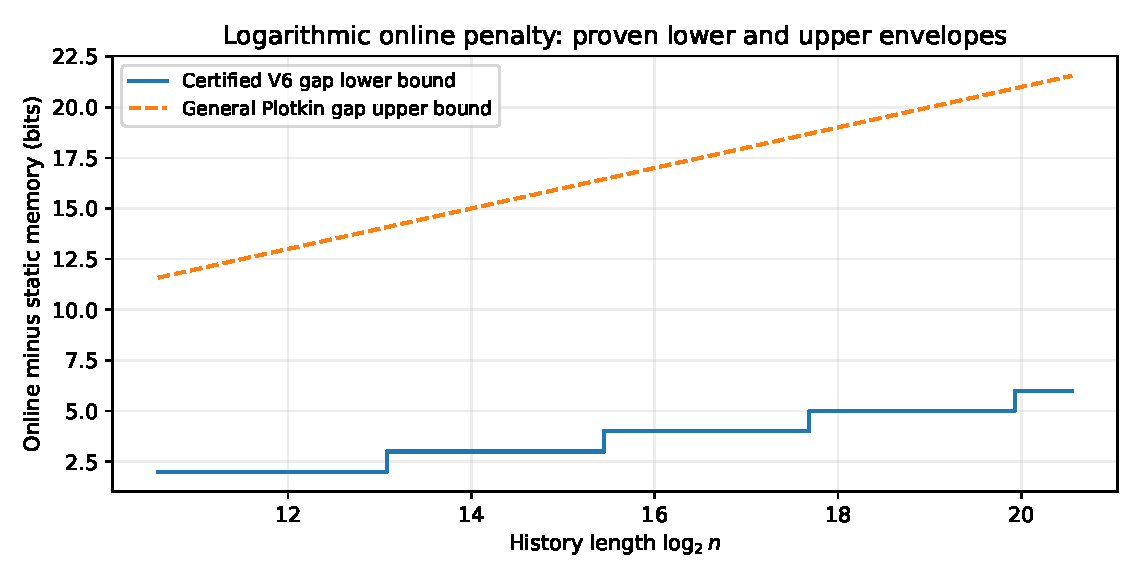
\includegraphics[width=.89\textwidth]{figures/v6_gap_envelopes.pdf}
\caption{Lower and upper bounds for the maximum online--static penalty in the $q>n/2$ parameter range. Steps correspond to the simplex-code dimension.}\label{fig:loggap}
\end{figure}

\subsection{Separation at every sufficiently large length}\label{subsec:alln}
Padding a simplex code extends the multiround separation to every sufficiently large length, with parameters satisfying $q>n/2$.
\begin{theorem}[Uniform logarithmic separation for all large $n$]\label{thm:alln}
For every integer $n\ge1536$ there exist integers $T,q$ with
\[
 1\le T,\quad n/2<q,\quad T+q<n,
 \quad T=o(n)\ \text{along the choices below},
\]
and a dimension $k=k(n)$ satisfying
\begin{equation}\label{eq:alln}
 R_T^{\rm on}(n,q)=n,\qquad
 \left\lceil\log_2\chi(Q_n^{T+q})\right\rceil\le n-k,
 \qquad k=\tfrac12\log_2n-O(\log\log n).
\end{equation}
Thus the gap grows logarithmically at every sufficiently large blocklength.
\end{theorem}
\begin{proof}
Let $k\ge2$ be the largest integer for which $n\ge32\cdot4^k(k+1)$. Set $r=2^k$, $T=4r(k+1)$ and divide $n=m(r-1)+a$, where $0\le a<r-1$. Since $r-1<r$,
\[
 m=\left\lfloor\frac n{r-1}\right\rfloor
 \ge\frac nr-1\ge 8T-1\ge7T,
 \qquad a<T.
\]
Define $d=mr/2$, $q=d-T-1$, and $s=d-1$. Clearly $s=T+q<n$ for $r\ge4$. Furthermore,
\[
 q-\frac n2=\frac{m-a}{2}-T-1
 \ge2T-1>0.
\]
The phase-$T$ minimum distance is $q+1=d-T>n/2$. The Plotkin estimate and the preceding bounds give
\[
 A(n,q+1)\le\frac{mr-2T}{m-a-2T}
 \le\frac{mr}{m-3T}\le\frac74r<2r,
\]
so $B_T<2r^2$. Since $d-(n-d+T)=m-a-T\ge m-2T$, we also have
\begin{align*}
 \ln\Gamma_T&\ge T\ln\left(\frac d{n-d+T}\right)
 =-T\ln\left(1-\frac{m-a-T}{d}\right)\\
 &\ge T\frac{m-a-T}{d}
 \ge\frac{2T}{r}\left(1-\frac{2T}m\right)
 \ge\frac{10T}{7r}=\frac{40}{7}(k+1).
\end{align*}
This strictly exceeds $\ln(2r^2)=(2k+1)\ln2$ for $k\ge2$, so Theorem~\ref{thm:amplified} again yields full online saturation.

For the static scheme, repeat each nonzero binary $k$-column $m$ times and append $a$ all-zero columns. The resulting $k$-dimensional binary linear code has every nonzero codeword of weight $d=mr/2=s+1$. Its cosets give the $n-k$ bit static coloring. Maximality of $k$ implies $n<32\cdot4^{k+1}(k+2)$, while its defining inequality implies $n\ge32\cdot4^k(k+1)$. These inequalities show $k=\frac12\log_2n-O(\log\log n)$ as $n\to\infty$. They also show $r\to\infty$, and $T/n\le1/(8r)\to0$.
\end{proof}

\begin{corollary}[Optimal order of the largest high-erasure online penalty]\label{cor:sharp}
For each $n$ define
\[
 G(n)=\max_{\substack{T\ge1,\ q>n/2\\T+q<n}}
 \left(R_T^{\rm on}(n,q)-\lceil\log_2\chi(Q_n^{T+q})\rceil\right).
\]
Then $G(n)=\Theta(\log n)$ as $n\to\infty$.
\end{corollary}
\begin{proof}
Theorem~\ref{thm:alln} provides an admissible $q>n/2$ construction with a logarithmic gap for every sufficiently large $n$. For the upper bound, a proper static color class has minimum distance at least $s+1>n/2$. Lemma~\ref{lem:plotkin} gives the bound $A(n,s+1)\le2n$. Since $2^n$ vertices must be covered, $\chi(Q_n^s)\ge2^n/(2n)$, whence its static cost is at least $n-\log_2(2n)$. Meanwhile the online encoder can always store the entire $n$-bit vector. Thus $G(n)\le\log_2(2n)$, proving the matching logarithmic order.
\end{proof}

\noindent For each phase $t$ and label $m$, write $D_{t,m}=C_{t,m}$ for the set of attainable current vectors.\par
\section{A distance-spectrum refinement of the multiround converse}\label{sec:spectrum}
\begin{theorem}[Pair-spectrum inequality]\label{thm:spectrum}
For every valid protocol and every integer $1\le t\le T$,
\begin{equation}\label{eq:spectrum}
\boxed{\quad
\sum_{m=1}^K\;\sum_{\{x,y\}\subset C_m}\binom{\dist(x,y)}{t}
\;\le\;
\sum_{m=1}^K\;\sum_{\{u,v\}\subset D_{t,m}}\binom{n-\dist(u,v)}{t}.
\quad}
\end{equation}
The sums are over unordered pairs of distinct binary vectors. No linearity, uniformity, or bounded computational-time assumption is imposed.
\end{theorem}
\begin{proof}
Take an unordered pair $\{x,y\}$ in one initial fiber, with differing-coordinate set $\Delta(x,y)$. Choose an unordered $t$-element subset $I\subseteq\Delta(x,y)$, update these coordinates in increasing order, and independently assign an arbitrary common value $b_i$ to each coordinate $i\in I$. This gives exactly $2^t\binom{\dist(x,y)}t$ labelled constructions: the terminal vectors $u=U_{I,b}(x)$ and $v=U_{I,b}(y)$ are still distinct because Lemma~\ref{lem:phase} gives $\dist(x,y)\ge T+q+1>t$. Both terminal executions have the same memory label by determinism. Hence each construction maps to a terminal label $m'$ and an unordered terminal pair $\{u,v\}\subset D_{t,m'}$.

Fix such an output $(m',\{u,v\})$ and write $h=\dist(u,v)$. In any preimage construction, all overwritten positions belong to the $n-h$ positions where $u$ and $v$ agree; there are at most $\binom{n-h}{t}$ choices for their set $I$. Once $I$ is fixed, its assigned values are determined by $u$ and $v$. Off $I$, the original two words are forced to equal $u$ and $v$. At each overwritten position they must be opposite; choosing which original word carries $1$ gives at most $2^t$ different unordered initial pairs. Each such pair, if admissible, has a unique initial label under $f$ and a deterministically determined output label. Thus every terminal labelled pair has at most $2^t\binom{n-h}{t}$ preimage constructions. Summing the preimage bound and cancelling $2^t$ proves~\eqref{eq:spectrum}.
\end{proof}

Define the distance-energy of a terminal code by
\[
\mathcal E_t(n,d)=\max_{\substack{\varnothing\ne C\subseteq\{0,1\}^n\\ \min_{u\ne v\in C}\dist(u,v)\ge d}}
\sum_{\{u,v\}\subset C}\binom{n-\dist(u,v)}{t}.
\]
For singleton codes the pair sum equals zero. Let $A(n,d)$ be the maximum size of a binary length-$n$ code of minimum distance at least $d$.
\begin{corollary}[Spectral cardinality bound]\label{cor:capacity}
Let $s=T+q<n$, $1\le t\le T$, and $z_m=|C_m|$. Then
\begin{equation}\label{eq:card}
\binom{s+1}{t}\sum_{m=1}^K\binom{z_m}{2}
\le K\,\mathcal E_t(n,s-t+1),
\end{equation}
where
\begin{equation}\label{eq:coarse}
\mathcal E_t(n,s-t+1)\le
\binom{A(n,s-t+1)}{2}\binom{n-s+t-1}{t}.
\end{equation}
Consequently, if $\binom{s+1}{t}>\mathcal E_t(n,s-t+1)$ for any $t\in[1,T]$, then $R_T^{\mathrm{online}}(n,q)=n$.
\end{corollary}
\begin{proof}
The first inequality follows from Theorem~\ref{thm:spectrum}, the initial minimum distance $s+1$, and the terminal minimum distance $s-t+1$. The second inequality bounds both the number of unordered terminal pairs and the weight of each pair. If $K\le2^{n-1}$, then $\sum_m\binom{z_m}{2}\ge\sum_m(z_m-1)_+\ge 2^n-K\ge K$, contradicting~\eqref{eq:card} under the asserted strict inequality. Storing the entire current $n$-bit vector is always feasible.
\end{proof}

\section{Parity-sensitive terminal capacity and improved saturation}\label{sec:parity}
The pair-spectrum inequality can exploit the parity of individual codewords. When the required terminal minimum distance is odd, a pair of words with the same parity has a stronger minimum-distance requirement than a pair of opposite parity. This yields a universal capacity bound with no linearity assumptions. We use the convention $\binom ab=0$ when $a<b$ or $b<0$.

\begin{lemma}[Parity-refined pair energy]\label{lem:parityenergy}
Let $C\subseteq\mathbb F_2^n$ be a binary code with $M=|C|$ and odd minimum distance $d\ge1$. For every integer $t\ge1$,
\begin{equation}\label{eq:parityenergy}
\begin{split}
\sum_{\{u,v\}\subset C}\binom{n-d_{\rm H}(u,v)}t
\ \le\ &\left\lfloor\frac{M^2}{4}\right\rfloor\binom{n-d}t\\
&+\left(\binom M2-\left\lfloor\frac{M^2}{4}\right\rfloor\right)\binom{n-d-1}t.
\end{split}
\end{equation}
The inequality is strict compared with the bound $\binom M2\binom{n-d}t$ whenever $M\ge3$ and $n-d\ge t$.
\end{lemma}
\begin{proof}
Partition $C$ according to even and odd Hamming weight, with classes of sizes $a$ and $b$, $a+b=M$. A pair from different classes is at odd distance, hence at distance at least $d$. A pair from the same class is at even distance, hence at distance at least $d+1$ because $d$ is odd. Since $h\mapsto\binom{n-h}t$ is nonincreasing on integral distances, the left side is at most
\[
 ab\binom{n-d}t+\left(\binom M2-ab\right)\binom{n-d-1}t.
\]
The coefficient of $ab$ is nonnegative and $ab\le\lfloor M^2/4\rfloor$, giving the claim. For $M\ge3$ the number $\binom M2-\lfloor M^2/4\rfloor$ is positive; when $n-d\ge t\ge1$, Pascal's identity makes the second binomial coefficient strictly smaller than the first.
\end{proof}

\begin{theorem}[Parity-sensitive saturation certificate]\label{thm:paritysat}
Fix $n\ge2$, $T\ge1$, $q\ge1$, $s=T+q<n$, and a round $1\le t\le T$. Suppose $d=s-t+1$ is odd. For any valid integer upper bound $A\ge A(n,d)$ define
\[
 \mathcal P_t(n,d,A)=\left\lfloor\frac{A^2}{4}\right\rfloor\binom{n-d}t+
 \left(\binom A2-\left\lfloor\frac{A^2}{4}\right\rfloor\right)\binom{n-d-1}t.
\]
Then the strict inequality
\begin{equation}\label{eq:paritycriterion}
\boxed{\quad\binom{s+1}t>\mathcal P_t(n,d,A)\quad}
\end{equation}
implies the exact online state cost
\[
\boxed{R_T^{\mathrm{on}}(n,q)=n.}
\]
The criterion holds for arbitrary deterministic nonlinear encoders and transitions.
\end{theorem}
\begin{proof}
For a terminal code $D$ of size $M\le A(n,d)\le A$, Lemma~\ref{lem:parityenergy} bounds its $t$-energy by the same expression with $M$ in place of $A$. This expression is nondecreasing as a function of the positive integer $M$: equivalently, it is the maximum of the nonnegative weighted pair count over all bipartitions of an $M$-element set, and adding a vertex cannot decrease that maximum. Consequently $\mathcal E_t(n,d)\le\mathcal P_t(n,d,A)$. Under \eqref{eq:paritycriterion}, Corollary~\ref{cor:capacity} excludes every protocol with at most $2^{n-1}$ private labels. The protocol retaining the current word has exactly $2^n$ states and proves equality.
\end{proof}

\begin{theorem}[Two interior exact online--static separations]\label{thm:interior}
The following two parameter triples lie strictly below the elementary saturation boundary $T+q>2n/3$ and satisfy
\[
\boxed{\ R_T^{\mathrm{on}}(n,q)=n,\qquad
\left\lceil\log_2\chi(Q_n^{T+q})\right\rceil=n-1:\ }
\]
\[
\boxed{(n,T,q)=(53,5,30)\qquad\text{and}\qquad(61,4,36).}
\]
In both cases the standard cardinality-only phase certificate combined with the binary Plotkin bound is inconclusive for every available phase, while \eqref{eq:paritycriterion} proves saturation.
\end{theorem}
\begin{proof}
For $(n,T,q)=(53,5,30)$ we have $s=35$, and choose $t=5$ and $d=s-t+1=31$. Plotkin gives
\[
 A(53,31)\le\left\lfloor\frac{62}{62-53}\right\rfloor=6.
\]
The two sides of the parity criterion satisfy the explicit integer inequality
\begin{equation}\label{eq:53}
\binom{36}{5}=376992>
9\binom{22}{5}+6\binom{21}{5}=359100.
\end{equation}
Theorem~\ref{thm:paritysat} proves $R_5^{\mathrm{on}}(53,30)=53$. For $(61,4,36)$ set $s=40$, $t=4$, $d=37$. Here Plotkin gives $A(61,37)\le\lfloor 74/13\rfloor=5$, and
\begin{equation}\label{eq:61}
\binom{41}{4}=101270>
6\binom{24}{4}+4\binom{23}{4}=99176.
\end{equation}
Thus $R_4^{\mathrm{on}}(61,36)=61$.

It remains to determine the static bit cost. At $n=53,s=35$, the initial minimum distance is $36$; Plotkin yields $A(53,36)\le\lfloor72/19\rfloor=3$. At $n=61,s=40$, the initial distance is $41$ and $A(61,41)\le\lfloor82/21\rfloor=3$. In either case a partition of the cube into $K$ codes of size at most three requires $K\ge\lceil2^n/3\rceil>2^{n-2}$, so at least $n-1$ static bits are required. The antipodal pairs give a proper coloring of $Q_n^s$ with exactly $2^{n-1}$ colors, since $s<n$. This establishes the matching static bit cost.

For the comparison with the older integer certificate, the unrefined Plotkin capacity at the chosen phase is $15\binom{22}{5}=395010$ for $n=53$, and $10\binom{24}{4}=106260$ for $n=61$, both larger than the corresponding left side. Direct substitution of the Plotkin upper bound into the other phases similarly fails to give a strict inequality; this is checked for all $1\le t\le T$ by the supplied exact-integer verifier. The new certificate is therefore strictly sharper in these two instances.
\end{proof}

\begin{table}[htbp]\centering\small
\begin{tabular}{@{}rrrrrrrr@{}}\toprule
$n$&$T$&$q$&$t$&Plotkin $A$&Initial pairs&Parity energy bound&Old energy bound\\\midrule
53&5&30&5&6&$376992$&$359100$&$395010$\\
61&4&36&4&5&$101270$&$99176$&$106260$\\\bottomrule
\end{tabular}
\caption{Integer certificates for the parity-sensitive capacity bound. The ``initial pairs'' column equals $\binom{T+q+1}t$. Online and static optimum costs are $n$ and $n-1$ bits, respectively.}\label{tab:parity}
\end{table}

\subsection{Association-scheme refinement of terminal energy}\label{sec:delsarte}
The parity bound admits a systematic refinement through the classical Delsarte inequalities~\cite{delsarte1973,macwilliams1977}. This replaces the scalar code-size term in the converse by a finite-dimensional feasible region.

For $0\le h,j\le n$ define the binary Krawtchouk polynomial
\[
K_h(j)=\sum_{a=0}^h(-1)^a\binom ja\binom{n-j}{h-a}.
\]
For a code $C$ with $M=|C|$, its ordered distance distribution is
\[
A_j(C)=\frac1M\bigl|\{(u,v)\in C^2:d_{\rm H}(u,v)=j\}\bigr|.
\]
Here $A_0=1$, $\sum_j A_j=M$, and $A_j=0$ for $1\le j<d$ when the minimum distance is at least $d$. Fourier orthogonality yields
\begin{equation}\label{eq:krawpositive}
\sum_{j=0}^n A_j(C)K_h(j)
=\frac1M\sum_{\substack{S\subseteq[n]\\|S|=h}}\left|\sum_{x\in C}(-1)^{\sum_{i\in S}x_i}\right|^2\ge0.
\end{equation}
The terminal energy is exactly
\begin{equation}\label{eq:delsarteenergy}
\sum_{\{u,v\}\subset C}\binom{n-d_{\rm H}(u,v)}t
=\frac M2\sum_{j=d}^n A_j(C)\binom{n-j}t.
\end{equation}
For each integer $M\le A(n,d)$, maximizing the right side over nonnegative real variables $A_d,\ldots,A_n$ subject to $\sum_{j=d}^n A_j=M-1$ and the $n$ inequalities \eqref{eq:krawpositive} therefore gives a valid upper bound on the energy of every $M$-word terminal code. Maximizing these linear-programming values over $1\le M\le A(n,d)$ gives a rigorous upper bound. A rational dual solution certifies the resulting bound. Substitution into Corollary~\ref{cor:capacity} incorporates pair-distance information; the two finite examples below admit simpler closed-form parity estimates.

\section{Two exact finite examples}
\begin{proposition}[Equality in the smallest nontrivial online example]\label{prop:n3}
There is a valid $(n,T,q)=(3,1,1)$ protocol with $K=4$ labels for which both sides of~\eqref{eq:spectrum} equal $12$. Moreover $K=4$ is optimal.
\end{proposition}
\begin{proof}
Initially group the eight vectors into four antipodal pairs $\{x,x\oplus111\}$. Each is a distance-$3$ code, and each pair contributes $\binom31=3$ to the left-hand side, totalling $12$. Upon any common overwrite, the two words in a pair differ in exactly two remaining positions and have equal parity, since two bits are flipped between them. The update rule can therefore save the parity of the updated vector as its terminal label; that parity is independent of which member of the initial pair was present. The two terminal fibers are the sets of four even- and odd-parity words. Each is a distance-$2$ code with six pairs, and every pair contributes $\binom{3-2}{1}=1$ to the right-hand side, totalling $12$. At either phase, revealing any two coordinates determines the third within the labelled fiber. Finally, the initial distance-$3$ requirement allows at most two words per label: $A(3,3)=2$. Eight words therefore need at least four labels.
\end{proof}

\begin{proposition}[A strict improvement over coarse terminal capacity]\label{prop:n5}
For binary codes of length five of minimum distance $3$,
\[
\boxed{\mathcal E_1(5,3)=10<12=\binom{A(5,3)}2(5-3).}
\]
\end{proposition}
\begin{proof}
First $A(5,3)=4$. Indeed, five codewords would give ten pairwise distances, each at least three, so their total pairwise distance would be at least $30$. In each of the five bit positions at most $2\cdot3=6$ of the ten word pairs can disagree, so the same total is at most $30$. Equality would force every pair to be at distance exactly three. This is impossible for any three binary words because the sum of their three pairwise Hamming distances is even. Conversely, the four codewords $0,7,25,30$ have minimum distance three.

For a four-word code, form the simple graph connecting pairs at distance exactly three. It is triangle-free by the same parity argument, so by Mantel's bound it has at most four of the six possible edges. Thus at least two pairs have distance at least four. The energy $\sum_{\{u,v\}}(5-\dist(u,v))$ is at most $4\cdot2+2\cdot1=10$. Three-word and smaller codes have energy at most $3\cdot2=6$. The four-code $\{0,7,25,30\}$ has pair distances $3,3,4,4,3,3$, attaining energy $10$. The coarse estimate gives $\binom42(5-3)=12$.
\end{proof}


\section{An explicit one-overwrite quotient code}\label{sec:one}
For one overwrite and one erased coordinate, a quotient-syndrome encoder gives a uniform construction with a closed-form decoder and a joint terminal representation of the overwrite coordinate and quotient syndrome.

Let $n\ge2$, $r=\lceil\log_2(n+1)\rceil$, and fix distinct nonzero $h_1,\dots,h_n\in\F^r$. Define the syndrome
\[
H(x)=\bigoplus_{j:x_j=1}h_j\in\F^r.
\]
For each coordinate $i$, let $G_i=\F^r/\langle h_i\rangle$ be the additive quotient by the two-element subgroup $\{0,h_i\}$, and write $[a]_i$ for the coset of $a$. Since $r\ge2$, choose a publicly defined $v_i\in\F^r\setminus\{0,h_i\}$; its class $[v_i]_i$ is nonzero. The group $G_i$ has $2^{r-1}$ elements.

The phase-zero memory is $H(x)$, occupying $r$ bits. At the unique blind update $(i,b)$, the machine sets
\begin{equation}\label{eq:oneupdate}
 M_1=\big(i,\ \beta=[H(x)]_i+b[v_i]_i\big).
\end{equation}
The updater computes the successor label from $H(x)$ and $(i,b)$. The state space at time one has $n2^{r-1}$ labels, with the announced overwrite value $b$ incorporated into the quotient class $\beta$. Under the update,
\[
[H(x)]_i=[H(y)]_i,
\]
since $H(y)-H(x)$ is a multiple of $h_i$. Thus the retained $\beta$ is a one-bit-shifted class of the \emph{present} word's syndrome. The decoder uses this class together with the visible coordinates.

\begin{theorem}[Uniform one-overwrite quotient theorem]\label{thm:one}
For all $n\ge2$,
\begin{equation}\label{eq:onebound}
\boxed{\quad
 R_1^{\rm on}(n,1)\le
 \min\left\{n,\ \lceil\log_2(n+1)\rceil-1+\lceil\log_2 n\rceil\right\}.
\quad}
\end{equation}
The encoder and decoder have uniform formulas, and updates use the stored label and the assigned coordinate--value pair.
\end{theorem}
\begin{proof}
The state \eqref{eq:oneupdate} uses $\lceil\log_2n\rceil+(r-1)$ bits. It remains to recover the unknown $y_j$ using the visible $y_{-j}$ and $(i,\beta)$.

If $j=i$, compute $\alpha=[H(y_{-i},0)]_i$ from all visible coordinates, where the erased bit is temporarily set to zero. Since the erased $i$th component only changes syndrome by $h_i$, $\alpha=[H(y)]_i$. By \eqref{eq:oneupdate}, $\beta=\alpha+y_i[v_i]_i$. The two possibilities $\alpha$ and $\alpha+[v_i]_i$ are distinct, so the decoder recovers $y_i$ exactly.

If $j\ne i$, the updated value $b=y_i$ is visible among the complementary coordinates. Hence the decoder obtains $\alpha=\beta+b[v_i]_i=[H(y)]_i$. Compute $\gamma=[H(y_{-j},0)]_i$ from the visible coordinates, temporarily setting the erased $j$th bit to zero. Then
\[
\alpha=\gamma+y_j[h_j]_i.
\]
As the columns are distinct and nonzero, $h_j\notin\langle h_i\rangle$ for $j\ne i$, so $[h_j]_i\ne0$. The two candidate values of $\alpha$ are distinct, giving a unique correct $y_j$. The decoder uses only the terminal label and supplied current complement. Recovery before the write is the ordinary one-erasure decoder for $H(x)$. The raw-state fallback costs $n$ bits and completes the bound.
\end{proof}

\begin{corollary}[Explicit logarithmic upper bound]\label{cor:one}
For all $n\ge2$,
\[
 \lceil\log_2(n+1)\rceil\le R_1^{\rm on}(n,1)
 \le\min\{n,\lceil\log_2(n+1)\rceil-1+\lceil\log_2n\rceil\}.
\]
Thus the single-overwrite problem has memory $\Theta(\log n)$, with an explicit factor approaching two between these general bounds. The lower bound is the radius-one Hamming packing bound from Theorem~\ref{thm:converse}.
\end{corollary}

\subsection{Seven-coordinate finite certificate}
When $n=7$, take $r=3$ and $h_i=i$ in the binary representation of $\F^3$. There are $7\cdot4=28$ phase-one labels, so the quotient theorem constructs a five-bit machine. The program \path{src/verify_one_step_family.py} enumerates every source, write, and query for $n=2,\dots,8$, including $128\times7\times2\times7=12,544$ combinations at $n=7$.

A 28-pair certificate, \path{certificates/n7_one_update_matching.json}, also describes a five-bit scheme using terminal independent sets. Its 56 initial-syndrome projection pieces $P_{i,b,[a]_i}=\{y:y_i=b,[H(y)]_i=[a]_i\}$ each have 16 words and are individually independent. The certificate pairs the pieces into 28 unions, each of which contains no two adjacent cube vertices. Because every possible $y$ consistent with an encoder label and overwrite event is within the matching union, the common terminal decoder is unambiguous. The separate checker \path{src/verify_n7_certificate.py} verifies every pairing and the same 12,544 triples using integer operations only. The quotient-code formula establishes the general construction; the matching certificate supplies a separate finite realization at $n=7$.

\subsection{Exact four-coordinate instance}
At $n=4$, a complementary-pair construction sharpens the generic quotient-code upper bound to the exact bit optimum.
\begin{proposition}[Four coordinates, one overwrite]\label{prop:n4}
$R_1^{\rm on}(4,1)=3$.
\end{proposition}
\begin{proof}
Initially store the unordered pair $\{x,\overline x\}$ as one of eight states. Given the update $(i,b)$, form the two possible current words $y=U_{i,b}(x)$ and $z=U_{i,b}(\overline x)$; they differ in exactly three positions and therefore have opposite overall parity. Store the unique even-parity member $e\in\{y,z\}$. There are eight possible even-parity words, which fit in three bits.

For any fixed state $e$, the true present word must lie in
\[
 \{e\}\ \cup\ \{e\oplus({\bf 1}\oplus e_i):i\in[4]\},
\]
where $e_i$ is the $i$th unit vector. The distance from $e$ to a nontrivial listed candidate is three; two different nontrivial candidates have distance two. Thus this set contains no adjacent words, and any one-erasure query is uniquely decodable. The stage-zero antipodal pair is likewise safe. The Hamming lower bound gives $R\ge\lceil\log_2 V(4,1)\rceil=3$, proving equality.
\end{proof}

The exact values for $(n,T,q)=(2,1,1),(3,1,1),(4,1,1)$ are respectively $2,2,3$. At $n=3$ the two-bit construction follows by an explicit antipodal-pair encoding with a phase-dependent decoder.


\section{Syndrome-compatible blind updates for general parity-check matrices}\label{sec:general-syndrome}
The exact one-write problem admits a useful reduction for initial encoders defined by a binary parity-check matrix. The next criterion distinguishes the existence of a one-coordinate witness from the stricter full-alphabet symmetry of the Hamming matrix. Throughout this section, let $H$ be an $r\times n$ binary matrix with pairwise distinct, nonzero columns $h_1,\ldots,h_n$. Assume that deleting any two columns leaves a matrix of rank $r$. This condition guarantees that every prescribed syndrome can be attained while any two coordinate values are fixed.

For $i\in[n]$, write $\mathscr L_i$ for the family of the $2^{r-1}$ affine pairs $L=\{a,a+h_i\}$ in $\mathbb F_2^r$. Define
\[
\mathcal A_{i,b,L}=\{y\in\mathbb F_2^n:y_i=b,\ Hy\in L\},\qquad
\mathscr H=\{h_1,\ldots,h_n\},
\]
and for two affine sets use $L+P=\{u+v:u\in L,\ v\in P\}$. Two distinct atoms are called \emph{incompatible} if their union contains a Hamming-distance-one pair. The initial syndrome encoder is $f_H(x)=Hx$.

\begin{theorem}[Column-set criterion for syndrome compatibility]\label{thm:column-criterion}
For distinct atoms $\mathcal A_{i,b,L}$ and $\mathcal A_{j,c,P}$, the following conditions are necessary and sufficient for incompatibility:
\begin{enumerate}[label=(\roman*),leftmargin=2em]
\item If $i\ne j$, then $(L+P)\cap\mathscr H\ne\varnothing$.
\item If $i=j$ and $b=c$ (hence $L\ne P$), then $(L+P)\cap(\mathscr H\setminus\{h_i\})\ne\varnothing$.
\item If $i=j$ and $b\ne c$, then $L=P$.
\end{enumerate}
Consequently, the one-overwrite terminal-label problem with initial encoder $f_H$ is exactly the vertex coloring problem for the explicitly specified graph in (i)--(iii). This graph may be constructed directly from the check columns and syndrome lines, with no enumeration of source words.
\end{theorem}
\begin{proof}
For every initial syndrome $s$, assigning $x_i\leftarrow b$ to all words in $C_s=\{x:Hx=s\}$ gives precisely $\mathcal A_{i,b,\{s,s+h_i\}}$: an updated word has one of those two syndromes, and the two possible old values at coordinate $i$ realize both cases. Since all columns are distinct and nonzero, every atom has minimum distance at least two. Thus two atoms can share a terminal label exactly when their union contains no distance-one pair.

Suppose first that $i\ne j$. If $y\in\mathcal A_{i,b,L}$ and $z\in\mathcal A_{j,c,P}$ satisfy $d_{\rm H}(y,z)=1$, then $z=y+e_k$ for some column index $k$, and $h_k=Hy+Hz\in L+P$. This proves necessity.

Conversely, take $h_k=u+v\in(L+P)\cap\mathscr H$ with $u\in L$ and $v\in P$. When $k\notin\{i,j\}$, select $y$ with $Hy=u$, $y_i=b$, and $y_j=c$. When $k=i$, select $y$ with the same syndrome and fixed coordinates $y_i=b$, $y_j=c$. When $k=j$, select $y$ with $Hy=u$, $y_i=b$, and $y_j=1-c$. The rank hypothesis guarantees that each of these selections exists. In every case $z=y+e_k$ belongs to $\mathcal A_{j,c,P}$ while $y$ belongs to $\mathcal A_{i,b,L}$. Thus the atoms are incompatible.

If $i=j$ and $b=c$, a Hamming-distance-one edge between the two atoms must flip some $k\ne i$. Exactly the same syndrome argument proves necessity of $h_k\in L+P$. Conversely, if such a $k$ exists, select $y$ with $Hy=u\in L$ and $y_i=b$ (possible by the rank hypothesis) and take $z=y+e_k$. This supplies the required edge. Finally, if $i=j$ and $b\ne c$, any edge must flip coordinate $i$. Its syndromes differ by $h_i$, so the corresponding syndrome lines must coincide. If $L=P$, choosing any $y$ in the first atom makes $y+e_i$ a member of the second, proving sufficiency.
\end{proof}

\begin{corollary}[One-column shortening preserves the exact conflict graph]\label{cor:shortened}
Let $r\ge3$ and let $H^-$ be the $r\times(2^r-2)$ matrix whose columns are all the nonzero elements of $\mathbb F_2^r$ except one arbitrary column. Write $n^-=2^r-2$ and $m=2^{r-1}$. For the fixed initial encoder $f_{H^-}(x)=H^-x$, the atom conflict graph is
\[
\boxed{\quad G^-_r\cong\bigvee_{i=1}^{n^-}(K_m\square K_2),\qquad
\chi(G^-_r)=n^-m.\quad}
\]
Consequently the minimum number of terminal labels is $(2^r-2)2^{r-1}$, and the optimum common initial/terminal storage budget is exactly
\[
\boxed{\quad R_1^{(H^-)}(2^r-2,1)=2r-1.\quad}
\]
The optimum is over all deterministic nonlinear update maps and decoders while the initial syndrome partition is held fixed.
\end{corollary}
\begin{proof}
Deleting a further two columns from $H^-$ leaves $2^r-4$ distinct nonzero columns. Every proper subspace contains at most $2^{r-1}-1$ nonzero vectors, and $2^r-4>2^{r-1}-1$ when $r\ge3$. Hence Theorem~\ref{thm:column-criterion} applies.

For $i\ne j$, $L+P$ is an affine plane with exactly four elements; at most one is zero and at most one is the deleted nonzero column. Thus it meets $\mathscr H$, and the two atoms are incompatible. For $i=j$, $b=c$, and $L\ne P$, the two-element set $L+P$ contains neither $0$ nor $h_i$, so deleting at most one nonzero column cannot eliminate all witnesses. These atoms are also incompatible. For opposite overwrite values at the same coordinate, incompatibility holds exactly when the syndrome lines coincide, by Theorem~\ref{thm:column-criterion}(iii). The resulting adjacency rule is therefore identical to that for the complete Hamming matrix.

For each coordinate the induced graph is $K_m\square K_2$, whose chromatic number is $m$ for $m\ge2$; different coordinate classes are completely joined. This proves $\chi(G^-_r)=n^-m$. A cyclic derangement of the $m$ colors between the two overwrite values gives an explicit coloring and therefore an executable update rule, as in Theorem~\ref{thm:optimal}. The initial phase uses only $2^r$ syndrome labels and $n^-m\ge 2^r$, so the same label alphabet serves both phases. Finally,
$2^{2r-2}< (2^r-2)2^{r-1}<2^{2r-1}$ for $r\ge3$, and taking the ceiling of the base-two logarithm gives $2r-1$ bits.
\end{proof}


\begin{proposition}[Cross-coordinate compatibility under affine-plane deletion]\label{prop:affine-deletion}
Let $r\ge4$, let $U\subseteq\mathbb F_2^r$ be a two-dimensional subspace, and choose $a\notin U$. Delete the four check columns in the affine plane $a+U$ from the complete Hamming matrix, leaving $n=2^r-5$ nonzero columns. The associated atom conflict graph has exactly
\[
\boxed{\quad 3\cdot2^{r+2}\quad}
\]
compatible unordered atom pairs whose overwritten coordinates are distinct. All such pairs involve distinct overwrite coordinates with check columns in $U\setminus\{0\}$. No other distinct-coordinate pair is compatible.
\end{proposition}
\begin{proof}
The two-column deletion rank condition holds, since the matrix retains $2^r-7>2^{r-1}-1$ nonzero columns after any further two deletions. For distinct coordinates $i,j$, Theorem~\ref{thm:column-criterion} states that their atoms are compatible exactly when the four-element affine plane $L+P$ contains no surviving check column. Every element other than zero and the deleted set belongs to the check-column set. Since $L+P$ has four elements, it can avoid the check columns only if it equals the removed plane $a+U$. In particular, its direction subspace must be $\operatorname{span}\{h_i,h_j\}=U$, so the two check directions are chosen from the three nonzero vectors of $U$. There are exactly three unordered such coordinate pairs.

Fix one of the three pairs. There are $2^{r-1}$ choices of the affine line $L$ of direction $h_i$. For each $L$ there are precisely two lines $P$ of direction $h_j$ with $L+P=a+U$: if $u\in L$, these are the two $h_j$-lines contained in the plane $a+u+U$. There are four independent choices of the assigned values $(b,c)$. Hence each coordinate pair supplies $2^{r-1}\cdot 2\cdot 4=2^{r+2}$ compatible unordered atom pairs, giving the asserted total.
\end{proof}

For $r=4$, this construction has $n=11$ coordinates and $176$ overwrite atoms; it produces $192$ compatible cross-coordinate pairs. Enumerating the $11\cdot2^{10}$ Hamming edges of the cube and all $\binom{176}{2}=15\,400$ atom pairs reproduces the criterion of Theorem~\ref{thm:column-criterion}. In this example, atoms from different overwrite coordinates can share a terminal label.

\begin{table}[htbp]\centering\small
\begin{tabular}{@{}rrrrr@{}}\toprule
$r$ & shortened length $n^-$ & initial syndromes & exact terminal labels & optimal bits \\\midrule
3&6&8&24&5\\
4&14&16&112&7\\
5&30&32&480&9\\
6&62&64&1,984&11\\
7&126&128&8,064&13\\\bottomrule
\end{tabular}
\caption{Exact successor-state costs for singly shortened Hamming check matrices. Six-coordinate verification covers each deleted column and all 1,128 unordered atom pairs.}\label{tab:shortened}
\end{table}

A chromatic refinement of this deletion appears in Section~\ref{sec:plane-exact}. The column-set criterion applies more broadly than the full and singly shortened Hamming families. In particular, deleting several check columns can remove all witnesses in $(L+P)\cap\mathscr H$ and create compatibility between atoms supported on different overwrite coordinates. The resulting graph determines the terminal state complexity conditional on the specified initial linear encoder.

\section{Exact atom coloring after affine-subspace puncturing}\label{sec:plane-exact}
Let $2\le d\le r-2$, let $U\le\mathbb F_2^r$ be a $d$-dimensional
linear subspace, and choose $a\notin U$. Delete the $2^d$ nonzero check
columns belonging to the affine coset $a+U$ from the full Hamming check
matrix. The resulting matrix $H_{a,U}$ has
\begin{equation}\label{eq:hierarchy-params}
 n=2^r-1-2^d,\qquad J=2^d-1,\qquad m=2^{r-1}
\end{equation}
columns. Exactly $J$ surviving columns lie in $U\setminus\{0\}$;
these are called \emph{exceptional}, while the other $n-J$ columns are
\emph{ordinary}. We continue to fix the initial encoder to
$f_{a,U}(x)=H_{a,U}x$ and optimize over all deterministic, possibly nonlinear,
terminal update and decoding rules. The initial syndrome partition remains fixed throughout this section.

\begin{theorem}[Affine-subspace puncturing hierarchy]\label{thm:plane-exact}
For all integers $r,d$ with $2\le d\le r-2$, the complete atom conflict
graph $G_{a,U}$ satisfies
\begin{equation}\label{eq:plane-exact}
 \boxed{\quad
 \chi(G_{a,U})=\left(n-\frac J2\right)m
 =\bigl(2n-2^d+1\bigr)2^{r-2},
 \qquad n=2^r-1-2^d.\quad}
\end{equation}
The minimum number of terminal memory labels for the fixed initial
syndrome is exactly this value, and the minimum common phase-zero/phase-one
bit budget is
\begin{equation}\label{eq:plane-bits}
 \boxed{\quad R_1^{(H_{a,U})}(2^r-1-2^d,1)=2r-1.\quad}
\end{equation}
The optimum includes nonlinear merging of overwrite atoms and
saves $Jm/2=(2^d-1)2^{r-2}$ terminal labels over the separate-coordinate
palette construction.
\end{theorem}
\begin{proof}
\emph{Rank and exact compatibility.}
After deleting any two further columns, $H_{a,U}$ retains
$2^r-2^d-3>2^{r-1}-1$ distinct nonzero columns because
$r\ge d+2$ and $d\ge2$. They span $\mathbb F_2^r$, and hence the
column-set criterion of Theorem~\ref{thm:column-criterion} applies.
For distinct overwritten coordinates $i,j$, the set $L+P$ is an affine
plane with four elements and direction space $\langle h_i,h_j\rangle$.
If it avoids the surviving check columns, every element belongs to
$\{0\}\cup(a+U)$. The possibility $0\in L+P$ is excluded: the three
nonzero points of a linear two-plane sum to zero, whereas a sum of three
points of $a+U$ lies in $a+U$ and is nonzero. Thus all four points lie in
$a+U$, so $h_i,h_j\in U$ and the two syndrome lines lie in U-cosets
$Q,Q+a$, respectively. Conversely, these conditions imply
$L+P\subseteq a+U$ and hence compatibility. We have proved
\begin{equation}\label{eq:hierarchy-cross}
 i\ne j:\quad \mathcal A_{i,b,L}\sim\mathcal A_{j,c,P}
 \ \Longleftrightarrow\ h_i,h_j\in U\setminus\{0\},\quad
 [L]_U+[P]_U=a+U,
\end{equation}
where $[L]_U$ is the containing coset of $U$, and $\sim$ denotes
compatibility.
For a fixed coordinate and equal assigned values, distinct syndrome lines
are compatible precisely when their sum avoids the surviving columns.
Since their two-point sum has nonzero difference $h_i$, this happens
exactly when $h_i\in U\setminus\{0\}$ and the two lines belong to mate
cosets $Q,Q+a$. For opposite assigned values, the corresponding atoms
are compatible exactly when their lines differ, as before.
Consequently, every ordinary-coordinate class induces
$K_m\square K_2$, and all the ordinary classes are completely joined to
one another and to the exceptional subgraph. Their exact contribution to
the chromatic number is $(n-J)m$.

\emph{Exceptional independent-set bound.}
Every pairwise compatible set of exceptional atoms contains
at most four atoms, uniformly in $r$ and $d$. If the atoms use just one
coordinate, then for either assigned value $b$ their syndrome lines must
lie in pairwise mate U-cosets. There can be at most two such lines, since
the involution $Q\mapsto Q+a$ admits no three pairwise mates, and two
different lines in the same U-coset at fixed $b$ conflict. Thus there
are at most two atoms per bit value and four in total.
If two or more overwritten coordinates occur, the cross-coordinate
criterion forces all atoms of a given coordinate to lie in the same
U-coset: every one of their cosets must be the unique mate of the coset
of any fixed atom from another coordinate. Distinct active coordinates
must therefore be assigned pairwise mate cosets, so there are at most two
active coordinates. Within one coordinate and one U-coset, at most one
atom with each assigned value can occur in a compatible set; hence each
coordinate contributes at most two atoms. Again the total is at most
four. Since there are $2Jm$ exceptional atoms, their chromatic number is
at least $2Jm/4=Jm/2$, giving
\[
 \chi(G_{a,U})\ge (n-J)m+Jm/2=(n-J/2)m.
\]

\emph{Exact four-atom coloring.}
Within every ordinary coordinate class, enumerate its $m$ syndrome lines
$L_0,\ldots,L_{m-1}$ and pair the atoms $(0,L_k)$ and
$(1,L_{k+1\bmod m})$ into one color. These two lines differ, so each
pair is compatible. Use disjoint palettes for all ordinary classes.

For the exceptional atoms, quotient the syndrome space by $U$. Translation
by $a+U$ partitions its $2^{r-d}$ cosets into $2^{r-d-1}$ mate pairs
$(Q,Q+a)$. Let $\ell=2^{d-1}\ge2$: every exceptional direction has
exactly $\ell$ syndrome lines within each U-coset. Enumerate these lines
in $Q$ and $Q+a$ separately, and pair their $b=0$ and $b=1$ atoms by
a cyclic derangement of the $\ell$ line indices. This produces exactly
$\ell$ compatible atom pairs per exceptional direction in each coset.
Enumerate the $J$ exceptional directions cyclically. For each mate pair
$(Q,Q+a)$, each direction $j$ and each line-pair index $k$, merge the
two-atom pair of direction $j$ from $Q$ with the two-atom pair of direction
$j+1\bmod J$ from $Q+a$. The four atoms are mutually compatible:
intra-coordinate compatibility comes from distinct lines and opposite
written values, and inter-coordinate compatibility follows from
\eqref{eq:hierarchy-cross}. Every exceptional atom occurs in exactly one
such group, so the number of colors needed per mate pair is $J\ell$.
Across all mate pairs this uses
$2^{r-d-1}J\ell=J2^{r-2}=Jm/2$ colors.
Together with the ordinary palettes, it attains the lower bound and
proves \eqref{eq:plane-exact}.

Finally, the initial syndrome requires $2^r$ labels, whereas
$\chi(G_{a,U})>2^{2r-2}\ge2^r$ under $r\ge d+2\ge4$.
The inequalities $2^{2r-2}<\chi(G_{a,U})<2^{2r-1}$ follow from
$2^{r-1}>3\cdot2^{d-1}+\frac12$ and
$n-J/2<2^r$. Therefore the least common bit budget is exactly $2r-1$.
\end{proof}

\begin{corollary}[Compatibility census for affine-coset deletion]\label{cor:plane-extra}
With $J=2^d-1$, the compatible atom pairs with distinct overwrite
coordinates number exactly
\begin{equation}\label{eq:cross-census}
 \boxed{\quad \binom J2 2^{r+d}.\quad}
\end{equation}
There are additionally exactly $J2^{r+d-2}$ compatible same-value
pairs supported on one exceptional coordinate. The total number of
compatible unordered atom pairs is
\begin{equation}\label{eq:all-census}
 \boxed{\quad nm(m-1)+J2^{r+d-2}+\binom J2 2^{r+d}.\quad}
\end{equation}
\end{corollary}
\begin{proof}
Fix an unordered pair of exceptional coordinates. Each of the $m$
syndrome lines in the first coordinate has exactly $\ell=2^{d-1}$
syndrome lines in the unique mate U-coset of the second coordinate.
Four independent choices of written values give $4m\ell=2^{r+d}$
compatible pairs, and there are $\binom J2$ coordinate pairs.
For a fixed exceptional coordinate and fixed written value, compatible
distinct lines must occupy mate cosets. There are $2^{r-d-1}$ mate pairs,
$\ell^2$ cross-coset choices per mate pair, and two written values,
yielding $2^{r-d}\ell^2=2^{r+d-2}$ such pairs per coordinate.
Finally, for every coordinate, opposite-value atoms on distinct syndrome
lines yield $m(m-1)$ compatible pairs, independently of the deleted set.
The three categories are disjoint.
\end{proof}

\begin{corollary}[Constant-fraction saving at maximal puncture dimension]
\label{cor:constant-fraction}
Choose $r=d+2$ and let $d\to\infty$. The exact fraction of terminal
labels saved relative to separate palettes is
\begin{equation}\label{eq:frac-saving}
\frac{nm-\chi(G_{a,U})}{nm}
 =\frac{2^d-1}{2(3\cdot2^d-1)}\longrightarrow\frac16.
\end{equation}
The reduction concerns the terminal alphabet cardinality; the minimum whole-bit budget in this family is $2r-1$.
\end{corollary}

\begin{table}[htbp]\centering\small
\begin{tabular}{@{}rrrrrrr@{}}\toprule
$r$ & $d$ & $n$ & overwrite atoms & separate colors & exact colors & saved labels\\\midrule
4 & 2 & 11 & 176 & 88 & 76 & 12\\
5 & 3 & 23 & 736 & 368 & 312 & 56\\
6 & 4 & 47 & 3,008 & 1,504 & 1,264 & 240\\
7 & 5 & 95 & 12,160 & 6,080 & 5,088 & 992\\\bottomrule
\end{tabular}
\caption{A double-parameter hierarchy of exact punctured-syndrome conflict graphs.
The first row recovers the four-column result. The $r=d+2$ sequence has
an asymptotic $1/6$ reduction in terminal labels, while the optimum whole-bit
count is $2r-1$. The accompanying program enumerates atom pairs for
$(r,d)=(4,2),(5,3),(6,4)$ and checks the stated color classes.}
\label{tab:plane-exact}
\end{table}

\section{Exact compatibility graphs for Hamming-syndrome initial memory}\label{sec:exactH}
For every coordinate $i$ and syndrome $s$, define the unordered affine line
\[
        L_i(s)=\{s,s+h_i\}\subseteq\mathbb F_2^r.
\]
For a fixed $i$, the $2^r$ syndromes are partitioned into $m=2^{r-1}$ such lines. Let $\mathscr L_i$ be the set of these $m$ lines. For $b\in\mathbb F_2$ and $L\in\mathscr L_i$, put
\[
   \mathcal A_{i,b,L}=\{y\in\mathbb F_2^n:y_i=b,\ Hy\in L\}.
\]

For this section set $n=2^r-1$, $r\ge3$. Let $H\in\mathbb F_2^{r\times n}$ have as columns all nonzero vectors of $\mathbb F_2^r$, indexed by $i\in[n]$. The fixed initial encoder is $f_H(x)=Hx$; its fibers $C_s=\{x:Hx=s\}$ are the cosets of the binary Hamming code. They have minimum distance three, so a single blind assignment followed by an erasure can be treated through the common-label update images. This section optimizes the terminal labels over arbitrary nonlinear updates while holding this initial partition fixed. Write $\mathscr L_i$ for the set of affine lines of direction $h_i$ in $\mathbb F_2^r$, and let $\mathcal A$ denote the family of overwrite atoms.

\begin{lemma}[Syndrome-pair collapse]\label{lem:atoms}
For every $s\in\mathbb F_2^r$, $i\in[n]$, and $b\in\mathbb F_2$,
\[
   U_{i,b}(C_s)=\mathcal A_{i,b,L_i(s)}.
\]
Each atom is a distance-two code. For fixed $i$, distinct lines give disjoint atoms at the same overwrite value $b$.
\end{lemma}
\begin{proof}
If $y=U_{i,b}(x)$ and $Hx=s$, then $y_i=b$ and $Hy=s$ or $s+h_i$, so the left side is contained in the right. Conversely, if $y_i=b$ and $Hy=s$, take $x=y$; if $Hy=s+h_i$, take $x=y+e_i$. In both cases $Hx=s$ and $U_{i,b}(x)=y$. If two words of one atom differed in one coordinate $j$, they would have syndrome difference $h_j$. Their common fixed $i$th value requires $j\ne i$, whereas two members of $L$ can differ only by $h_i$; contradiction. The last statement is immediate because the $L\in\mathscr L_i$ partition the syndrome space.
\end{proof}

Thus the initial $2^r\cdot2n$ labeled update requests collapse into exactly $2nm=n2^r$ \emph{distinct update atoms}. A final memory label may receive multiple atoms if and only if their union has minimum distance at least two. For fixed $f_H$, therefore, the minimum terminal label count equals the chromatic number of the \emph{atom conflict graph}: atoms are vertices and two vertices are adjacent exactly when their union contains a pair of words at Hamming distance one. This equivalence allows terminal codes to be nonlinear and arbitrarily shaped.

\subsection{The full conflict graph}
\begin{lemma}[Robust full rank]\label{lem:rank}
For $r\ge3$, deleting any two columns from $H$ leaves a matrix of rank $r$.
\end{lemma}
\begin{proof}
There remain $2^r-3$ distinct nonzero $r$-vectors. A proper subspace of $\mathbb F_2^r$ contains at most $2^{r-1}-1$ nonzero vectors, and $2^r-3>2^{r-1}-1$ for $r\ge3$. Therefore the remaining columns span $\mathbb F_2^r$.
\end{proof}

\begin{theorem}[Complete atom incompatibility law]\label{thm:adj}
For two \emph{distinct} atoms $\mathcal A_{i,b,L}$ and $\mathcal A_{j,c,L'}$, with $r\ge3$, they are incompatible precisely in the following cases:
\begin{enumerate}[label=(\roman*),leftmargin=2em]
\item $i\ne j$;
\item $i=j$ and $b=c$ (necessarily $L\ne L'$);
\item $i=j$, $b\ne c$, and $L=L'$.
\end{enumerate}
Equivalently, two distinct atoms are compatible if and only if they have the same overwritten coordinate, opposite assigned values, and different syndrome lines.
\end{theorem}
\begin{proof}
\emph{Different coordinates $i\ne j$.} Choose any $a\in L$ and $a'\in L'$. The four differences between points of $L$ and $L'$ form the coset
\[
       (a+a')+\operatorname{span}_{\mathbb F_2}\{h_i,h_j\},
\]
which has four distinct elements. Since $\{0,h_i,h_j\}$ has only three elements, some difference is a nonzero column $h_k\notin\{h_i,h_j\}$. Choose the corresponding $u\in L$ and $v\in L'$ with $u+v=h_k$. By Lemma~\ref{lem:rank}, we can choose $y$ satisfying $Hy=u$, $y_i=b$, and $y_j=c$: the other $n-2$ columns still span $\mathbb F_2^r$. Let $z=y+e_k$. Then $z$ and $y$ are adjacent, while $z_j=c$ and $Hz=v$. Hence $y\in\mathcal A_{i,b,L}$ and $z\in\mathcal A_{j,c,L'}$, proving incompatibility.

\emph{Same coordinate and same assigned value.} The lines $L,L'$ are disjoint. Choose $u\in L$, $v\in L'$. The difference $u+v$ is nonzero and cannot equal $h_i$; it must be $h_k$ for some $k\ne i$. Since the columns other than $i$ span $\mathbb F_2^r$, choose $y$ with $y_i=b$ and $Hy=u$, and put $z=y+e_k$. Then $z_i=b$ and $Hz=v$, giving an adjacent pair in the two atoms.

\emph{Same coordinate and opposite values.} Every edge between their atoms must flip coordinate $i$, because the prescribed values at $i$ are opposite. Such a flip changes the syndrome by $h_i$, so its two endpoints lie in the same $i$-line. Therefore different lines $L\ne L'$ are compatible. If $L=L'$, choose $y$ with $y_i=b$ and $Hy\in L$; then $y+e_i$ belongs to the atom with assigned value $1-b$ and the same line, proving incompatibility.
\end{proof}

Recall that the \emph{join} of graphs connects every vertex of each component to every vertex of the other components, while $G\square H$ denotes the Cartesian product of graphs.
\begin{corollary}[Exact graph structure and chromatic number]\label{cor:chi}
Let $G_r$ be the atom conflict graph for $f_H$. With $m=2^{r-1}$,
\[
\boxed{\quad G_r\cong \bigvee_{i=1}^{n}\left(K_m\square K_2\right),
\qquad \chi(G_r)=nm=(2^r-1)2^{r-1}.\quad}
\]
The graph has $2nm$ vertices and $nm^2+\binom n2(2m)^2$ edges.
\end{corollary}
\begin{proof}
Theorem~\ref{thm:adj} makes distinct coordinate classes completely joined. Inside one coordinate class, all atoms with fixed $b$ form a clique $K_m$, and opposite-$b$ vertices are adjacent exactly when their line indices agree. Hence this component is $K_m\square K_2$. It requires at least $m$ colors because one $b$-class is a clique. Conversely, use $m$ colors on $b=0$ indexed by line, and a derangement of these colors on $b=1$; for $m\ge2$, a cyclic shift is a derangement. Thus its chromatic number is $m$. Since the palettes of joined components must be disjoint, the total is $nm$. The edge count follows from $m^2$ edges inside each coordinate class and $(2m)^2$ cross-edges per pair of coordinate classes.
\end{proof}

\subsection{Sharp terminal-state cost and synthesis}
\begin{theorem}[Sharp conditional one-overwrite optimum]\label{thm:optimal}
Let $n=2^r-1$ with $r\ge3$, and require the initial encoder to be $f_H(x)=Hx$. Among \emph{all} deterministic (possibly nonlinear) updates and terminal single-erasure decoders with no external update log, the minimum number of phase-one labels equals
\[
\boxed{\quad \kappa^{(H)}_{\mathrm{terminal}}(n,1)=n2^{r-1}.\quad}
\]
The minimum common label budget across phases is the same. Consequently, the \emph{conditional} bit optimum is
\[
\boxed{\quad R_1^{(H)}(2^r-1,1)=2r-1.\quad}
\]
\end{theorem}
\begin{proof}
For any initial syndrome $s$ and overwrite $(i,b)$, the complete set of possible resulting current words is the atom $\mathcal A_{i,b,L_i(s)}$, by Lemma~\ref{lem:atoms}. Since the transition cannot observe the initial word inside the syndrome fiber, it must map this entire atom to one terminal label. If two atoms are mapped to the same label, their union must permit zero-error recovery of one erased coordinate, equivalently it must have minimum distance at least two. Hence these atoms must receive a proper coloring of $G_r$. Corollary~\ref{cor:chi} requires at least $nm$ terminal labels, irrespective of nonlinearity.

For attainability, enumerate $\mathscr L_i$ as $L_{i,0},\ldots,L_{i,m-1}$. Use the same $m$ terminal colors for the two overwrite values, but pair $\mathcal A_{i,0,L_{i,k}}$ with $\mathcal A_{i,1,L_{i,k-1}}$, with indices modulo $m$. Their lines differ because $m\ge2$; Theorem~\ref{thm:adj} shows their union is a distance-two code. Give this union the label $(i,k)$, with $0\le k<m$. For initial syndrome $s$, let $a$ be the index of $L_i(s)$. On update $(i,b)$, store $(i,a)$ if $b=0$ and $(i,a+1\pmod m)$ if $b=1$. In either case, the actual updated word belongs to its labeled union.

The decoder receives the label $(i,k)$ and all but one coordinate of $y$. It tests the two possible completions of the erased bit, accepting the unique one with $y_i=0$ and $Hy\in L_{i,k}$, or $y_i=1$ and $Hy\in L_{i,k-1}$. Existence follows from the transition invariant; uniqueness follows because the labeled union is a distance-two code. At phase zero, $Hx$ and the $n-1$ visible coordinates already recover the missing bit. Since $nm\ge 2^r$ for $n\ge3$, the shared label alphabet of size $nm$ serves both phases. Finally, $\lceil\log_2(nm)\rceil =2r-1$ because $2^{r-1}\le n<2^r$. This proves both exact assertions.
\end{proof}

The algorithm operates directly on syndrome representatives. An initial syndrome is computed in $O(nr)$ bit operations, each update maps the stored syndrome and overwrite parameters to a terminal label using $O(r)$-bit arithmetic, and the final decoder checks two completions using an $O(nr)$-bit syndrome computation. Storage is exactly $2r-1$ bits after reserving unused binary labels. The phase index itself is public and carries no update-dependent data.


Let $X=\{0,1\}^n$. A nonempty $S\subseteq X$ is a $d$-code template when $d_{\rm H}(u,v)\ge d$ for all distinct $u,v\in S$. Write $\mathcal C_d(X)$ for the finite family of such subsets, and let $d_t=q+T-t+1$. For $i\in[n]$ and $b\in\{0,1\}$, $U_{i,b}(S)=\{U_{i,b}(x):x\in S\}$.
\section{Temporal code-template synthesis}\label{sec:template}
\begin{theorem}[Temporal template covers]\label{thm:cover}
A zero-error protocol with at most $K$ memory labels exists if and only if there are families $\mathcal F_0,\ldots,\mathcal F_T$ satisfying
\begin{enumerate}[label=(\roman*),leftmargin=2em]
\item $\mathcal F_t\subseteq\mathcal C_{d_t}(X)$, and $1\le|\mathcal F_t|\le K$ for all $t$;
\item $\bigcup_{S\in\mathcal F_0}S=X$;
\item for each $t<T$, $S\in\mathcal F_t$, and $(i,b)\in[n]\times\{0,1\}$, there is $D\in\mathcal F_{t+1}$ with $U_{i,b}(S)\subseteq D$.
\end{enumerate}
Each such family specifies an encoder, deterministic update tables for all $T$ phases, and decoders. The characterization holds for general deterministic protocols.
\end{theorem}
\begin{proof}
For necessity, take at each phase the distinct nonempty exact attainable sets $S_{t,m}$. Lemma~\ref{lem:phase} gives (i). The initial fibers cover $X$, giving (ii). Every allowed update from state $m$ goes to a fixed new label $m'$, so the full image $U_{i,b}(S_{t,m})$ lies inside $S_{t+1,m'}$, giving (iii).

For sufficiency, label at most $K$ templates separately at each phase; labels may be reused because $t$ is public. For input $x$, choose any template $S\in\mathcal F_0$ containing $x$ and store its label. For any label corresponding to $S$ and update $(i,b)$, choose one containing successor template $D$ promised by (iii) and set the next label to $D$. Arbitrarily define transitions on unused labels. By induction, the current vector always lies in the currently labeled template. Given $E$ and the unerased coordinates, exactly one vector in this template agrees with the observation: existence follows from the invariant, while two such vectors would differ only on $E$, violating its minimum distance at least $d_t\ge q+1$. Hence the decoder is well-defined and correct.
\end{proof}

\begin{corollary}[Exact finite geometric optimization]\label{cor:kappa}
Writing $\mathfrak T(n,T,q)$ for the finite collection of sequences of template families satisfying (i)--(iii),
\[
\boxed{\ \kappa_T(n,q)=\min_{(\mathcal F_0,\ldots,\mathcal F_T)\in\mathfrak T(n,T,q)}\max_{0\le t\le T}|\mathcal F_t|\ .\ }
\]
Evaluating this finite combinatorial optimization gives the exact state count; Theorem~\ref{thm:cover} then constructs an optimal online protocol.
\end{corollary}

\subsection{Dominance, maximality, and induced-cube codes}
For a fixed future family $\mathcal F$ define the \emph{safe predecessor family}
\[
\mathsf W_t(\mathcal F)=\left\{S\in\mathcal C_{d_t}(X):
\forall(i,b)\ \exists D\in\mathcal F\ U_{i,b}(S)\subseteq D\right\}.
\]
This family is downward closed among nonempty subsets: any nonempty subset of a safe template is safe. Let $\operatorname{Max}\mathsf W_t(\mathcal F)$ be its inclusion-maximal members. At the terminal phase set $\operatorname{Max}\mathsf W_T$ to the family of inclusion-maximal $(q+1)$-code templates in $X$.

\begin{theorem}[Maximal-safe normal form]\label{thm:max}
If a $K$-label protocol exists, then families in Theorem~\ref{thm:cover} may be selected so that
\begin{enumerate}[label=(\alph*),leftmargin=2em]
\item every $\mathcal F_t$ is an antichain under set inclusion;
\item $\mathcal F_T\subseteq\operatorname{Max}\mathsf W_T$;
\item for $t<T$, every $S\in\mathcal F_t$ belongs to $\operatorname{Max}\mathsf W_t(\mathcal F_{t+1})$.
\end{enumerate}
Consequently, testing the existence of a $K$-label protocol reduces to backward choices among maximal-safe predecessor sets.
\end{theorem}
\begin{proof}
Begin with any covering witness from Theorem~\ref{thm:cover}. First enlarge each terminal template to a maximal $(q+1)$-code, leaving its label unchanged. This preserves incoming image containments and validity of the terminal decoder. Now work backward. For fixed already-enlarged $\mathcal F_{t+1}$, each $S\in\mathcal F_t$ belongs to $\mathsf W_t(\mathcal F_{t+1})$: all its former successor templates have been enlarged. Since the ground cube is finite and safety is downward closed, extend $S$ to an inclusion-maximal member $\widehat S\in\mathsf W_t(\mathcal F_{t+1})$. Replacing each template by such an extension preserves all predecessor image containments, the initial coverage if $t=0$, and all outgoing safety conditions. Removing duplicate extended sets can only decrease the number of labels. Inclusion-maximal members of the same downward-closed family form an antichain. Induct backward through phase zero. The resulting families satisfy all three properties without increasing $K$.
\end{proof}

There is a constructive way to enumerate the maxima in this theorem. For a choice map $\sigma:[n]\times\{0,1\}\to\mathcal F$, define
\[
V_\sigma=\bigcap_{i=1}^n\bigcap_{b\in\{0,1\}}
\bigl\{x\in X:U_{i,b}(x)\in\sigma(i,b)\bigr\}.
\]
\begin{proposition}[Induced-cube enumeration]\label{prop:induced}
Every maximal member of $\mathsf W_t(\mathcal F)$ is a maximal independent set in the graph $Q_n^{d_t-1}[V_\sigma]$ induced on $V_\sigma$ for at least one of the $|\mathcal F|^{2n}$ possible maps $\sigma$. Conversely, all such independent sets are safe, and retaining their inclusion-maximal members over all $\sigma$ gives precisely $\operatorname{Max}\mathsf W_t(\mathcal F)$.
\end{proposition}
\begin{proof}
For any safe $S$, choose a valid successor template $\sigma(i,b)$ separately for each of the $2n$ update inputs. Then $S\subseteq V_\sigma$, and $S$ is independent in the indicated induced graph. If $S$ is maximal safe but can be enlarged as a code inside $V_\sigma$, that larger set is also safe under the same successor selection, a contradiction. Conversely, any independent subset of $V_\sigma$ is a $d_t$-code and maps into its assigned successor under all updates, hence is safe. Maximalizing over all maps, then discarding inclusion-dominated results, is therefore exact.
\end{proof}


\section{Quantitative comparisons and finite certificates}
Table~\ref{tab:bounds} compares the sphere lower bound, the greedy-coloring/dictionary bound, and the explicit moment/dictionary bound. All entries use integer bounds. The one-step column follows the quotient-code construction, with a separate finite certificate at $n=7$. The moment construction has polynomial-time encoding and decoding; the greedy-coloring construction may use a nonuniform exponential-size table.

\begin{table}[htbp]
\centering\small
\begin{tabular}{rrrrrrl}
\toprule
$n$&$T$&$q$&Packing lower&Greedy upper&Moment upper&One-step / exact\\
\midrule
3&1&1&2&3&3&$2$ (the three-coordinate case)\\
4&1&1&3&4&4&$3$ (exact)\\
5&1&1&3&5&5&$4$ (exact; finite certificate)\\
7&1&1&3&7&7&$\le5$ (verified)\\
15&1&1&4&12&15&$\le7$\\
31&1&1&5&15&18&$\le9$\\
63&1&1&6&18&21&$\le11$\\
31&2&2&9&27&31&---\\
63&3&2&11&42&54&---\\
127&4&3&19&65&84&---\\
\bottomrule
\end{tabular}
\caption{Guaranteed charged bits; lower is valid for all deterministic schemes, whereas each upper is achieved by a specified construction. The $n=4$ and $n=5$ values are exact; exhaustive checks cover the $n=7$ quotient construction and its matching certificate.}\label{tab:bounds}
\end{table}

\begin{figure}[htbp]
\centering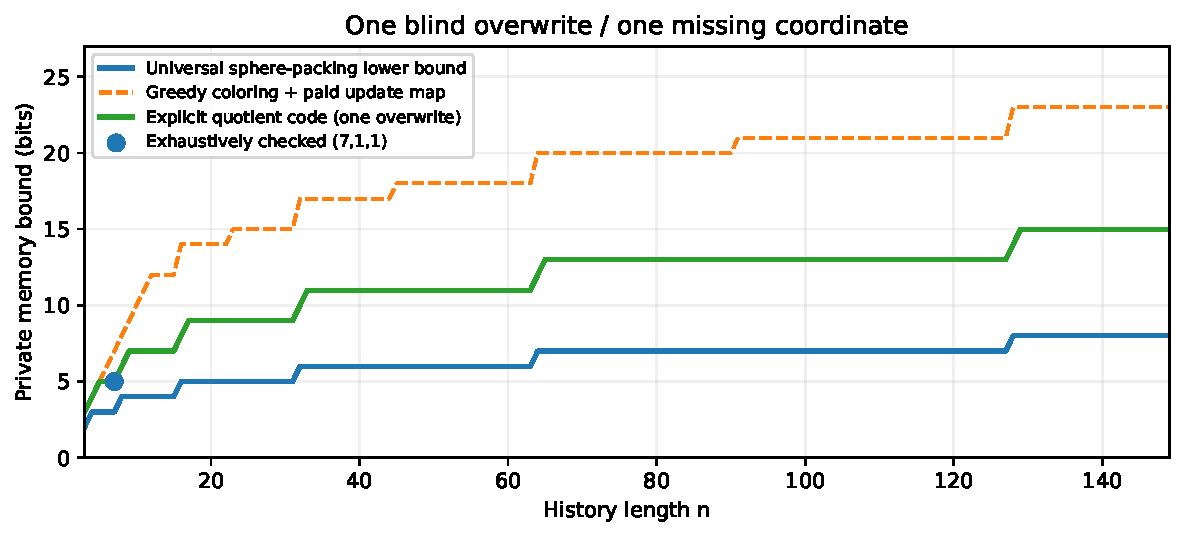
\includegraphics[width=.91\textwidth]{figures/bounds_T1_q1.pdf}
\caption{Bounds for $T=q=1$, including the analytic quotient-code upper bound and a five-bit protocol at $n=7$ checked by finite enumeration. The plotted gap is between the general converse and the one-write upper bound.}\label{fig:bounds}
\end{figure}

\paragraph{Finite checks.} Finite tests cover 8,128 parameter pairs for the volume bounds, all update--query instances of the quotient encoder for $2\le n\le8$, the 28-pair seven-coordinate certificate, and 1,750 Vandermonde update--recovery trials. See Appendix~\ref{app:computation} for the corresponding programs.


\section{Conclusion}
The incidence converse identifies the saturation threshold $T+q\ge\lceil n/2\rceil+1$. For $n=4(2^k-1)$, replicated simplex codes establish an exact $k$-bit difference between online and zero-update storage after a single blind assignment. Column completion extends a logarithmic gap to every sufficiently large blocklength.

For longer update horizons, pair amplification and distance spectra give additional converse bounds. At fixed syndrome partitions, affine-subspace deletion gives exact terminal-state chromatic numbers. The template-cover formulation expresses finite-horizon protocols as compatible families of error-correcting codes.

\appendix

\section{Bit-level state accounting and dictionary ranking}
The charged private map is a partial function $d:S\to\{0,1\}$ with $|S|\le T$. Its number of possibilities is exactly
\[
D_T(n)=\sum_{k=0}^{\min(T,n)}\binom nk2^k.
\]
A combinatorial ranking implements the charged private map: order the subsets first by their size $k$ and then in colexicographic order, and order the bit assignments on a fixed subset as binary integers. Write $S=\{a_1<\cdots<a_k\}\subseteq\{0,\ldots,n-1\}$ in zero-based coordinates. Its colex rank is
\[
 \mathrm{colex}(S)=\sum_{j=1}^k\binom{a_j}{j}.
\]
The map's index is
\begin{equation}\label{eq:maprank}
\mathrm{rank}(d)=\sum_{j=0}^{k-1}\binom nj2^j
  + 2^k\mathrm{colex}(S)+\sum_{j=1}^{k}d(a_j)2^{j-1}.
\end{equation}
As $S$ varies over the $\binom nk$ $k$-element sets and its values over $2^k$ assignments, the last two terms cover the entire block of $\binom nk2^k$ consecutive integers. The first term places this block after all smaller cardinalities. Therefore \eqref{eq:maprank} is a bijection between all private maps and $\{0,\ldots,D_T(n)-1\}$, which is representable in exactly $\lceil\log_2D_T(n)\rceil$ bits. The inverse rank algorithm, including the binomial-coefficient search for each $a_j$, requires polynomial time in $n,T$. The ranking formula is enumerated over 1,424 eligible maps by \texttt{src/packing.py}.

In the one-update theorem, identify $\F^r$ with the integers $0,\ldots,2^r-1$ and let $p_i$ be the position of the highest nonzero bit of $h_i$. Each orbit $\{a,a\oplus h_i\}$ has a unique representative with bit $p_i$ equal to zero: the numerically smaller element. Delete that bit to rank the orbit in $\{0,\ldots,2^{r-1}-1\}$. The phase-one state becomes the single integer
\[
 \mathrm{index}(i,\beta)=(i-1)2^{r-1}+\mathrm{rank}_{G_i}(\beta),
\]
using exactly $\lceil\log_2(n2^{r-1})\rceil$ binary places. The resulting integer specifies the complete stored label. Reversible ranking is checked over 20,036 labels.

\section{Phase information and state accounting}
The phase $t\in\{0,\ldots,T\}$ is public, and the decoder may depend on $t$. The transition receives the current label and the next coordinate assignment. A time-homogeneous variant can simulate the phase-aware protocol by storing a phase counter of $\lceil\log_2(T+1)\rceil$ bits alongside the summary. The stated optima use the public-phase convention.

The coalesced partial map stores the most recent assigned value at each edited coordinate; its complete range of values is included in the state budget. A variant imposing secrecy of the edited-coordinate set would have a different characteristic graph.

\section{First-phase incidence verification}
The program \path{verify_global_incidence.py} checks the identities in Lemma~\ref{lem:incidence}, simplex weights, Plotkin bounds, and the parameter inequalities of Theorem~\ref{thm:onewrite-alln}. For initial pairs in dimensions four through eight, it enumerates the distinct one-write images and their mutual distances.

A deterministic conditional-expectation choice of the additional columns is implemented in \path{construct_completed_simplex.py}. After any prefix, the conditional expected exponential potential is proportional to $\sum_{u\ne0}e^{-\theta S_u}$, where $S_u$ counts columns selected so far on which the nonzero linear functional $u$ evaluates to one and $\theta=4(m/2-2)/a$. Choosing the next nonzero column $v$ to maximize
\[
 \sum_{u\ne0:\,u\cdot v=1}e^{-\theta S_u}
\]
minimizes the next conditional expectation. Its initial value is below one by the union bound in Theorem~\ref{thm:onewrite-alln}; consequently the completed generator satisfies the required minimum-weight inequalities. The program evaluates the selection scores numerically and checks the final codeword weights by exact integer arithmetic.

\section{Computational verification}\label{app:computation}
The reproduction suite covers the general bounds, finite protocols, multiround inequalities, and successor-atom graphs:
\begin{enumerate}[label=(\roman*),leftmargin=2em]
\item \texttt{src/verify\_bounds.py}: every $(n,s)$ with $2\le s\le n\le128$, using $T=s-1$ to maximize the dictionary upper bound at fixed $s$, for 8,128 checked pairs;
\item \path{src/verify_one_step_family.py}: all sources, coordinate/value writes and final erased coordinates for each $2\le n\le8$, including the 12,544 seven-coordinate triples;
\item \path{src/verify_n7_certificate.py}: a second seven-coordinate encoding based on 28 precomputed pairs of cube-independent pieces, including direct pairwise distance checks;
\item \texttt{src/verify\_n4\_exact.py}: 512 four-coordinate write--query triples, together with all phase-zero observations, for the three-bit antipodal construction;
\item \texttt{src/packing.py}: exact reversible ranking for 1,424 private maps and 20,036 quotient labels, with no floating-point comparisons;
\item \texttt{src/bounds\_and\_moments.py}: seven parameter settings with 250 seeded cases each, checking the modular moment update-and-recovery implementation;
\item \path{src/verify_saturation.py}: exact Hamming-triangle checks for all triples through $n=7$ and 101 complete translated-pair partition checks for $4\le n\le10$, including explicit forced-edge multiplicities and phase-one capacity counts;
\item \path{src/verify_multiround_amplification.py}: 52 parameter instances auditing all unordered source pairs and canonical $t$-step overwrites, including the exact multiplicity bound;
\item \texttt{src/verify\_log\_separation.py}: 23 exact large-integer comparisons for the logarithmic-gap subsequence and all-length family, with a CSV certificate. The plotted envelopes are stored as vector figures, and plot generation is separate from the mathematical verification.
\item \path{verify_affine_plane_exact.py}: exact atom conflict comparisons at $r=4,5$ and an optional $r=6$ full-column check, including explicit optimal coloring, a $2^{11}$-word independent cube-edge witness audit, and every one-write/single-erasure observation in the $r=4$ case;
\item \path{verification/verify_parity_upgrade.py}: an independent enumeration of all 120 four-word, distance-three codes of length five and exact integer evaluations of the two new interior online-saturation certificates. Every phase is also checked against the older Plotkin/cardinality certificate.
\end{enumerate}
The 28-pair JSON certificate records a seven-coordinate matching. Its pairs are checked by distance enumeration, and the quotient formula supplies the general construction. The scripts use the Python standard library.



\begin{thebibliography}{99}\small
\bibitem{shannon1956} C. E. Shannon, ``The zero error capacity of a noisy channel,'' \emph{IRE Transactions on Information Theory} \textbf{2} (1956), 8--19. DOI: \href{https://doi.org/10.1109/TIT.1956.1056798}{10.1109/TIT.1956.1056798}.
\bibitem{hamming1950} R. W. Hamming, ``Error detecting and error correcting codes,'' \emph{Bell System Technical Journal} \textbf{29} (1950), 147--160.
\bibitem{plotkin1960} M. Plotkin, ``Binary codes with specified minimum distance,'' \emph{IRE Transactions on Information Theory} \textbf{6} (1960), 445--450. DOI: \href{https://doi.org/10.1109/TIT.1960.1057584}{10.1109/TIT.1960.1057584}.
\bibitem{ahlswede1975} R. Ahlswede and J. K\"orner, ``Source coding with side information and a converse for degraded broadcast channels,'' \emph{IEEE Transactions on Information Theory} \textbf{21} (1975), 629--637. DOI: \href{https://doi.org/10.1109/TIT.1975.1055469}{10.1109/TIT.1975.1055469}.
\bibitem{witsenhausen1976} H. S. Witsenhausen, ``The zero-error side information problem and chromatic numbers,'' \emph{IEEE Transactions on Information Theory} \textbf{22} (1976), 592--593. DOI: \href{https://doi.org/10.1109/TIT.1976.1055607}{10.1109/TIT.1976.1055607}.
\bibitem{wynerziv1976} A. D. Wyner and J. Ziv, ``The rate-distortion function for source coding with side information at the decoder,'' \emph{IEEE Transactions on Information Theory} \textbf{22} (1976), 1--10.
\bibitem{macwilliams1977} F. J. MacWilliams and N. J. A. Sloane, \emph{The Theory of Error-Correcting Codes}, North-Holland, Amsterdam, 1977.
\bibitem{delsarte1973} P. Delsarte, \emph{An Algebraic Approach to the Association Schemes of Coding Theory}, Philips Research Reports Supplements 10, 1973.
\bibitem{orlitsky2001} A. Orlitsky and J. R. Roche, ``Coding for computing,'' \emph{IEEE Transactions on Information Theory} \textbf{47} (2001), 903--917. DOI: \href{https://doi.org/10.1109/18.915643}{10.1109/18.915643}.
\bibitem{koulgi2003} P. Koulgi, E. Tuncel, S. L. Regunathan, and K. Rose, ``On zero-error source coding with decoder side information,'' \emph{IEEE Transactions on Information Theory} \textbf{49} (2003), 99--111. DOI: \href{https://doi.org/10.1109/TIT.2002.806154}{10.1109/TIT.2002.806154}.
\bibitem{bakshi2010} M. Bakshi and M. Effros, ``On zero-error source coding with feedback,'' \emph{Proceedings of IEEE ISIT} (2010), 11--15. DOI: \href{https://doi.org/10.1109/ISIT.2010.5513304}{10.1109/ISIT.2010.5513304}.
\bibitem{charpenay2024} N. Charpenay, M. Le Treust, and A. Roumy, ``Side information design in zero-error coding for computing,'' \emph{Entropy} \textbf{26} (2024), article 338. DOI: \href{https://doi.org/10.3390/e26040338}{10.3390/e26040338}.
\bibitem{ostergard2004} P. R. J. {\"O}sterg{\aa}rd, ``On a hypercube coloring problem,'' \emph{Journal of Combinatorial Theory, Series A} \textbf{108} (2004), 199--204. DOI: \href{https://doi.org/10.1016/j.jcta.2004.06.010}{10.1016/j.jcta.2004.06.010}.
\bibitem{jiangvardy2004} T. Jiang and A. Vardy, ``Asymptotic improvement of the Gilbert--Varshamov bound on the size of binary codes,'' \emph{IEEE Transactions on Information Theory} \textbf{50} (2004), 1655--1664. DOI: \href{https://doi.org/10.1109/TIT.2004.831751}{10.1109/TIT.2004.831751}.
\bibitem{mazumdar2012} A. Mazumdar, G. W. Wornell, and V. Chandar, ``Update efficient codes for error correction,'' \emph{Proceedings of IEEE ISIT} (2012), 1558--1562. DOI: \href{https://doi.org/10.1109/ISIT.2012.6283534}{10.1109/ISIT.2012.6283534}.
\bibitem{mazumdar2014} A. Mazumdar, V. Chandar, and G. W. Wornell, ``Update-efficiency and local repairability limits for capacity-approaching codes,'' \emph{IEEE Journal on Selected Areas in Communications} \textbf{32} (2014), 976--988. DOI: \href{https://doi.org/10.1109/JSAC.2014.140517}{10.1109/JSAC.2014.140517}.
\bibitem{sin2020} P. Sin, J. Sorci, and Q. Xiang, ``Linear representations of finite geometries and associated LDPC codes,'' \emph{Journal of Combinatorial Theory, Series A} \textbf{173} (2020), 105238. DOI: \href{https://doi.org/10.1016/j.jcta.2020.105238}{10.1016/j.jcta.2020.105238}.
\bibitem{chandran2014} N. Chandran, B. Kanukurthi, and R. Ostrovsky, ``Locally updatable and locally decodable codes,'' \emph{Theory of Cryptography Conference}, Lecture Notes in Computer Science (2014). DOI: \href{https://doi.org/10.1007/978-3-642-54242-8\_21}{10.1007/978-3-642-54242-8\_21}.
\bibitem{nakkiran2014} P. Nakkiran, N. B. Shah, and K. V. Rashmi, ``Fundamental limits on communication for oblivious updates in storage networks,'' \emph{IEEE GLOBECOM} (2014). DOI: \href{https://doi.org/10.1109/GLOCOM.2014.7037161}{10.1109/GLOCOM.2014.7037161}.
\bibitem{kokkala2018} J. I. Kokkala and P. R. J. {\"O}sterg{\aa}rd, ``The chromatic number of the square of the 8-cube,'' \emph{Mathematics of Computation} \textbf{87} (2018), 2551--2561. DOI: \href{https://doi.org/10.1090/mcom/3291}{10.1090/mcom/3291}.
\bibitem{ghosh2021} S. Ghosh, P. Krishnan, and L. P. Natarajan, ``Blind updates in coded caching,'' \emph{IEEE Journal on Selected Areas in Information Theory} (2021). DOI: \href{https://doi.org/10.1109/JSAIT.2021.3126603}{10.1109/JSAIT.2021.3126603}.
\bibitem{li2023} T. Li, J. Liang, H. Yu, and R. Zhou, ``Tight cell-probe lower bounds for dynamic succinct dictionaries,'' preprint (2023), \url{https://arxiv.org/abs/2306.02253}.
\bibitem{cohen1997} G. Cohen, I. Honkala, S. Litsyn, and A. Lobstein, \emph{Covering Codes}, North-Holland Mathematical Library 54, Amsterdam, 1997.
\bibitem{shen2025} Z. Shen, Y. Cai, K. Cheng, P. P. C. Lee, X. Li, Y. Hu, and J. Shu, ``A survey of the past, present, and future of erasure coding for storage systems,'' \emph{ACM Transactions on Storage} \textbf{21} (2025), Article 4, 39 pp. DOI: \href{https://doi.org/10.1145/3708994}{10.1145/3708994}.
\bibitem{domingues2026} G. M. Domingues, ``Compressing dynamic fully indexable dictionaries in Word-RAM,'' preprint (2026), \url{https://arxiv.org/abs/2603.23119}.
\bibitem{matsuta2022} T. Matsuta and T. Uyematsu, ``An equivalent expression for the Wyner--Ziv source coding problem,'' \emph{IEICE Transactions on Fundamentals of Electronics, Communications and Computer Sciences} \textbf{E105-A} (2022), 353--362. DOI: \href{https://doi.org/10.1587/transfun.2021TAP0005}{10.1587/transfun.2021TAP0005}.
\bibitem{malak2022} D. Malak, ``Fractional graph coloring for functional compression with side information,'' in \emph{2022 IEEE Information Theory Workshop (ITW)} (2022). DOI: \href{https://doi.org/10.1109/ITW54588.2022.9965814}{10.1109/ITW54588.2022.9965814}.
\end{thebibliography}

\end{document}
